\documentclass[tesis,reqno]{unaltesis2}

%reqno es para q los numeros de las ecuaciones salgan a la derecha leqno es para la izquierda

%unaltesis 2 lines
\makeatletter
%\deactivatetilden
\makeatother

\usepackage{listings}
\usepackage{amsmath,amssymb,setspace}
\usepackage{graphicx}
\usepackage{stackrel}
\usepackage[bookmarks]{hyperref}
\usepackage{setspace}
%\usepackage[ruled, vlined,boxed,commentsnumbered,shortend]{algorithm2e}
\usepackage{algorithm2e}
%\usepackage[ruled,vlined]{algorithm2e}
%\usepackage{minitoc}
\usepackage{caption}
\usepackage{subcaption}
\usepackage{amsthm}
% \usepackage{epstopdf}
\usepackage{lscape}

%%Es mejor usar \newcommand que \def. El primero hace ciertas validaciones
\newcommand\deq{\stackrel{{}_{\delta}{}}{\raisebox{-0.4ex}[+0.5ex][-8.2ex]{$=$}}}
\newcommand\g{\stackrel{{}_{\gamma}{}}{\raisebox{-0.4ex}[+0.5ex][-8.2ex]{$=$}}}
\newcommand\dg{\stackrel[]{\delta\gamma}{=}}
%\def\dg{\stackrel{{}_{\delta}{}_{\gamma}}{\raisebox{-0.4ex}[-0.4ex][-8.2ex]{$=$}}}
\newcommand\pd{\stackrel{{}_{\delta}}{\raisebox{0.6ex}[-0.4ex][-8.2ex]{$\leadsto$}}}
\newcommand\pg{\stackrel{{}_{\gamma}}{\raisebox{0.6ex}[-0.4ex][-8.2ex]{$\leadsto$}}}
\newcommand\pdg{\stackrel{{}_{\delta}{}_{\gamma}}{\raisebox{0.6ex}[-0.4ex][-8.2ex]{$\leadsto$}}}

%% Enviroment to theorems
\newtheorem{theorem}{Theorem}[section]
\newtheorem{lemma}[theorem]{Lemma}
\newtheorem{proposition}[theorem]{Proposition}
\newtheorem{corollary}[theorem]{Corollary}

\begin{document}
%%%%%%%%%%%%%%%%%%%%%%%%%%%%%%%%%%%%%%%%%%%%%%%%%%%%%%%%%%%%%%%%%%%%%%%%%%%%%%%%%%%%%%%%%%%%%%%%%%%%%%%%%%%%%%%%%
%Title page

%\Titulo{A hybrid evolutionary algorithm for vehicle routing problem with stochastic demands}
%\Titulo{A hybrid local rollout dynamic programming global evolutionary algorithm for the vehicle routing problem with stochastic demands}
\Titulo{A hybrid dynamic programming - evolutionary algorithm for vehicle routing problem with stochastic demands}

\Autor{Robinson A. Jaque P.}

\CodigoAutor{299800}

\AnoGrado{2011}

\MesGrado{Junio}

\Grado{Master of Sciences}

\Programa{Computer Science}

\Facultad{Engineering}

\Departamento{Computer and Industrial Engineering}

\Sede{Bogota D.C.}

\Tutor{Germ\'an Hern\'andez, Ph.D.}

\TituloTutor{Associated Professor}

\JuradoA{1, Ph.D.}

\JuradoB{2, Ph.D.}

\JuradoC{Member 3 of the Jury}

\NumeroDeJurados{2}

%%%%%%%%%%%%%%%%%%%%%%%%%%%%%%%%%%%%%%%%%%%%%%%%%%%%%%%%%%%%%%%%%%%%%%%%%%%%%%%%%%%%%%%%%%%%%%%%%%%%%%%%%%%%%%%%%
%PRELIMINARY PAGES
\maketitle \Preliminares \PaginaDeAprobacion

\onehalfspacing
%%%%%%%%%%%%%%%%%%%%%%%%%%%%%%%%%%%%%%%%%%%%%%%%%%%%%%%%%%%%%%%%%%%%%%%%%%%%%%%%%%%%%%%%%%%%%%%%%%%%%%%%%%%%%%%%%
%ABSTRACT
\begin{resumen}
In this work we propose a hybrid dynamic programming-evolutionary algorithm to solve the vehicle routing problem with stochastic demands, it is a well known NP-hard problem where uncertainty enhances the computational efforts required to obtain a feasible and near-optimal solution. We develop an evolutionary technique where a rollout dynamic programming algorithm is applied as local search method to improve the quality of solutions. Motivated by computational considerations, the rollout algorithm can be applied partially, so, this finds competitive solutions in large instances for which the global rollout dynamic programming strategy is time unfeasible.
\\
\end{resumen}

%%%%%%%%%%%%%%%%%%%%%%%%%%%%%%%%%%%%%%%%%%%%%%%%%%%%%%%%%%%%%%%%%%%%%%%%%%%%%%%%%%%%%%%%%%%%%%%%%%%%%%%%%%%%%%%%%
%ACKNOWLEDGEMENTS
\begin{Reconocimientos}
Last thing to do :-)\\

\end{Reconocimientos}

%%%%%%%%%%%%%%%%%%%%%%%%%%%%%%%%%%%%%%%%%%%%%%%%%%%%%%%%%%%%%%%%%%%%%%%%%%%%%%%%%%%%%%%%%%%%%%%%%%%%%%%%%%%%%%%%%
%DEDICATION
\begin{Dedicatoria}
To Hari
\end{Dedicatoria}


%%%%%%%%%%%%%%%%%%%%%%%%%%%%%%%%%%%%%%%%%%%%%%%%%%%%%%%%%%%%%%%%%%%%%%%%%%%%%%%%%%%%%%%%%%%%%%%%%%%%%%%%%%%%%%%%%
%TABLE OF CONTENTS
\tableofcontents

%%%%%%%%%%%%%%%%%%%%%%%%%%%%%%%%%%%%%%%%%%%%%%%%%%%%%%%%%%%%%%%%%%%%%%%%%%%%%%%%%%%%%%%%%%%%%%%%%%%%%%%%%%%%%%%%%
%LIST OF FIGURES
\listoffigures

%%%%%%%%%%%%%%%%%%%%%%%%%%%%%%%%%%%%%%%%%%%%%%%%%%%%%%%%%%%%%%%%%%%%%%%%%%%%%%%%%%%%%%%%%%%%%%%%%%%%%%%%%%%%%%%%%
%LIST OF TABLES
\listoftables

%%%%%%%%%%%%%%%%%%%%%%%%%%%%%%%%%%%%%%%%%%%%%%%%%%%%%%%%%%%%%%%%%%%%%%%%%%%%%%%%%%%%%%%%%%%%%%%%%%%%%%%%%%%%%%%%%
%LIST OF SYMBOLS
\chapter*{Notation}
\label{chap:notation}

\begin{table}
 \begin{tabular}{|c|l|}
  \hline
  \textbf{Symbol} & \textbf{Definition}\\
  \hline
  $n$ & Number of customers\\
  $d_{ij}$ & Distance between a pair of customers $i$ and $j$\\
  $E[L_{\tau}]$ & Expected distance of an apriori solution (base sequence) $\tau$\\
  $l$ & Location of vehicle\\
  $q_l$ & Vehicle capacity when customer $l$ has already been served.\\
  $p_i(j)$ & Probability of customer $i$ take the demand value $j$\\
  $K$ & Maximal demand\\
  $\bar{D}_i$ & Maximal demand of customer $i$\\
  $Q$ & Maximal capacity of vehicle\\
%Chapter 3 - Genetic algorithm

  \hline
 \end{tabular}

\end{table}


%%%%%%%%%%%%%%%%%%%%%%%%%%%%%%%%%%%%%%%%%%%%%%%%%%%%%%%%%%%%%%%%%%%%%%%%%%%%%%%%%%%%%%%%%%%%%%%%%%%%%%%%%%%%%%%%%
%%%%%%%%%%%%%%%%%%%%%%%%%%%%%%%%%%%%%%%%%%%%%%%%%%%%%%%%%%%%%%%%%%%%%%%%%%%%%%%%%%%%%%%%%%%%%%%%%%%%%%%%%%%%%%%%%
%Document body
\CuerpoDeLaTesis

%////////////////////////////////////////////////////////////////////////////////////////////////////////////////
 \chapter{Introduction}
\label{chap:intro}


\section{Introduction}

The classic problem about vehicle routing (VRP) is an well known \textit{NP-hard} ~\cite{Lenstra_1981} optimization problem of importance in different logistics, it consist in delivery goods to a set of costumers geographically dispersed, using a fleet of vehicles that begin its route in the central depot. The problem consists in to assign to each vehicle a route with the objective of minimizing the transportation cost.

The cost generated in the transport of goods, like the size of the fleet of vehicles maintenance, combustible, and so on, are significant owing to the transport processes are involved at all stages of production processes, accounting for 10\% to 20\% of the final product cost~\cite{toth_vehicle_2001}.

One of the first investigation that studied the vehicle routing problem was in the year 1959, in that work Dantzing and Ramser~\cite{Dantzing1959} analyzed an oil dispatching problem with trucks, that problem arise as a generalization of the classic traveling salesman problem (TSP), where the salesman has to visit a set of costumers only one time, and then come back to the origin point, building a Hamiltonian road on the graph consisting of customers (vertices) and the possible paths between clients (edges).

Different variations of the VRP have been proposed with the aim of approaching the problem real contexts; these problems include the addition of variables and constraints. The figure below shows a diagram with the most popular variants of VRP.

\begin{figure}[!htbp]
  \begin{center}
    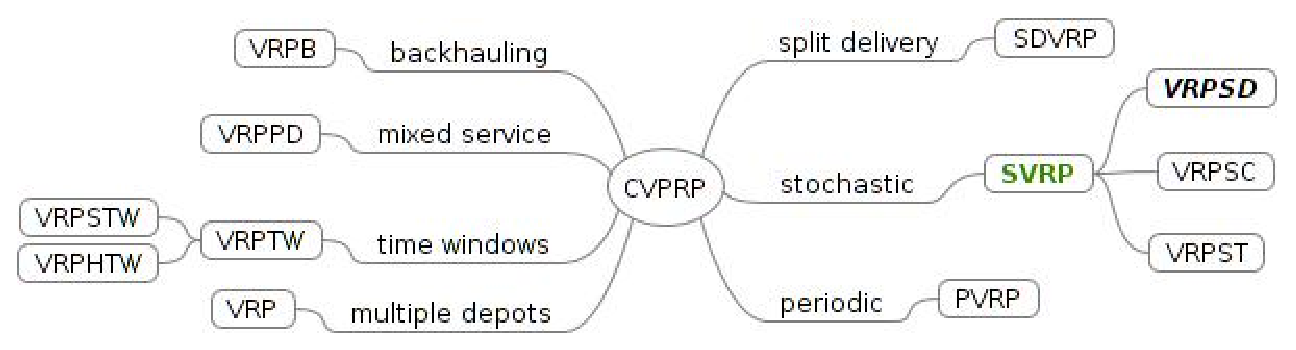
\includegraphics[width=0.8\textwidth]{Images/Chapter1/variants_vrp.eps}
  \end{center}
  \caption{Basic variants of the Vehicle Routing Problem}
  \label{fig:VRP_variants}
\end{figure}

When vehicles capacity is fixed origin the CVRP (Capacited Vehicle Routing Problem); if there are many depots, then we have MDVRP (Multiple Deposit Vehicle Routing Problem). The SDVRP (Split delivery Vehicle routing problem) is a relaxation of the problem that allows a costumer be served by several vehicles, being important in cases where the customer demand exceeds the vehicle capacity. Generally the VRP provide a planning for a fixed period, the PVRP (Periodic Vehicle Routing Problem) provides that planning for $m$ periods.

One of the most studied variants of the problem is caused by including time windows for deliveries, VRPTW (Vehicle Routing Problem with Time Windows), for this problem can be considered hard time windows (VRTHTW) that can't be done delivery outside the established periods, and soft time windows (VRPSTW) in which deliveries can be made outside these periods with a penalty.

The problems that include pick-up and delivery can be divided in VRPB (Vehicle Routing Problem with Backhauls) and VRPPD (Vehicle Routing Problem with Pick-Up and Delivery) in the VRPB the group of costumers is divided in two subgroups, for the first group all pick-up's are made of some product, then the vehicle return to the depot, then the deliveries are realized to the second group of costumers.  In the VRPPD the pick-up's and deliveries to customers are made simultaneously.

The SVRP (Stochastic vehicle routing problem) arise when there is uncertainty about some of the components of the VRP, i.e. one or more variables are random, usually these problems include VRPSC (Vehicle routing problem with stochastic costumers) that include random customers, the VRPST (Vehicle Routing Problem with Stochastic Times) where travel times are random and VRPSD (Vehicle Routing Problem with Stochastic Demands), where the customers' demands are known only with a probability distribution.

The SVRP's differ from the deterministic VRP in many important aspects. The solution concept is different, many properties of the deterministic problem are not manageable in the stochastic case and solution methodologies are considerably more complex, often SVRP is considered a computationally intractable problem and only small instances can be solved optimally and algorithms are difficult to design and evaluate~\cite{gendreau_stochastic_1996}.

The SVRP is either often modeled in the framework of stochastic programming (optimization) integer or mixed or as a Markov decision process. In stochastic programming, problems are usually modeled as two-stage usually as chance constrained program (CCP) or as a stochastic program with recourse (SPR).

The VRPSD is an open problem of great importance in logistics owing to the diversity of real situations it represents, this problem occur in the delivery of home heating oil~\cite{dror_computational_1985} in which each customer maintains a local inventory of the product and consumes a amount of oil each day, therefore each day a fleet of trucks is dispatched to resupply a subset of customers, stochastic demands are also evident in the collection of money by the vehicles of values, e.g. is touched off when collect money by a central bank~\cite{jianhua_fan_multiple_2006} from several but not all of its branches every day, the capacity of the vehicle used may be constrained for an upper bound on the amount of money that a vehicle might carry for safety reasons. The distribution of demand at each certain branch may be different, associated with the amount of money it handles. Other VRPSD arise in delivering the post to large customers~\cite{Markovic_2005}, vending machines~\cite{yang_stochastic_2000} or delivering medical supplies in response to large-scale emergency~\cite{dessouky_rapid_2006}, in recycling and waste management, among others.

\section{Proposal}

Design a hybrid evolutionary algorithm which combine stochastic dynamic optimization operators to find solutions for the vehicle routing problem with stochastic demands, moreover evaluate the algorithm performance.


\section{Objective}

Design and test a hybrid evolutionary algorithm + stochastic dynamic optimization (SDO) operators for the vehicle routing problem with stochastic demands.

\subsection{Specifics Objectives}

\begin{enumerate}
 \item Analyze the alternatives for modeling and representing problem, and selected the most computationally convenient.
 \item Design evolutionary and stochastic dynamic optimization operators algorithm to solve VRPSD.
 \item Implement the designed algorithm.
 \item Select benchmarking problems instances and alternative algorithms for testing.
 \item Develop experimental analyses and comparisons.
\end{enumerate}

\section{Contributions}

The evolutionary algorithms haven't been broadly used to solve the vehicle routing problem with stochastic demands, thus a hybrid evolutionary algorithm which combine stochastic dynamic optimization operators is proposed, it contribute with a new methodology to deal with the problem.

\section{Outline}

In this first chapter was carried out a summary of the issues to be addressed, in chapter 2 presents the background and is presented the state of the art of the VRPSD, chapter 3 presents the Methodology used and presents the proposed algorithm, the chapter 4 presents the experiments, the numerical results and compare and discuss the results comparing with the outcomes obtained by other authors, finally in chapter 5 presents the conclusions of the study.



%Outline
%1. Introduction
%2. Preliminars
%3. Stochastic dynamic programming algorithms
%4. Memetic algorithm
%5. Results 
%6. Conclusions and open problems
%7. Bibliography

%//Preliminars
 \chapter{Background}
\label{chap:backgroud}
%\minitoc

In this chapter, we carry out a specialized literature review of VRPSD, and point out applications and methodologies used to deal with it. Moreover, we examine modeling approaches to this problem in order to exploit the structure and solution properties following the methodology proposed, focusing on the stochastic dynamic programming (SDP) approach, where we first show a dynamic programming background before presenting the SDP formulation for VRPSD.

%\minitoc %mini table of contets for the chapter

\section{A review of Vehicle Routing Problem with Stochastic Demands}

In recent years the literature related to the stochastic vehicle routing problem has grown du to its application to real life problems, as well as to the academic interest in studying the problem theoretically. Consequently, a number of solutions have been proposed to deal with these problems.

\subsection{Application cases}

There are many applications of the VRPSD. In a huge number of real situations, the customer demand is unknown and its probability distribution can only be estimated. Eventhough, in spite of the fact that the demand can be known in many cases, when the vehicle arrives to the customer, the demand value changes, e.g., delivering petroleum products or industrial gases (Chepuri and Homem-De-Mello~\cite{Chepuri}). To ilustrate these cases, we focus on the problem where gas stations are placed geographically dispersed and a fuel transport vehicle is entrusted to deliver a fuel quantity determined when the vehicle arrives at the customer location; the demand is unknown since despite the remaining fuel was known at the time to make the order, when the vehicle arrives after this time, the fuel stock has decreased.

In the case of Automatic Teller Machines (ATM), not only the daily demand for cash is uncertain, but the maximal amount of cash that may be picked up by trucks for money transportation is also limited for security and insurance reasons.

\subsubsection*{The Traveling Repairman Problem (TRP)} 

This problem was introduced by Bertsimas and Van Ryzin~\cite{bertsimas_stochastic_1991} in 1991; they analyzed the mathematical model for dynamic and stochastic VRP with the dynamic TRP. In that model, the objective is to minimize the average time demands in the system. 

That problem is presented when a machine breaks down and must be repaired, in order to achieve such objective, it is important  to know the distance between the starting point and the arrival point, the urgency of the situation (hight or low), the availability of the repairman, etc. A real example of that problem is on electric power company, which has to travel point by point  to fix the problems that can suddenly arise; the problem has the characteristics of increased costumer, and the time spent in fixing the problems variates according to the particular environment.

Many authors have studied the problem; Jothi and Raghavachari~\cite{jothi_approximatingk-traveling_2007} analyze two algorithms to solve the problem; in 1993 Das and Wortman~\cite{Tapas} studied the TRP with a single repairman, and they  proposed a probability model that is useful for evaluating the system performance measures, such as the inactivity time, the availability of a machine and of the repairman.  

\subsubsection*{Currier mail services} 

Nowadays, there are many companies that offer the service of pick-up packages or mail and delivery of goods to the point where the costumer indicates; this problem, becomes dynamic because the driver unknow where will the next pick-up or quantity or volume of goods take place.

In 2004 Timon \textit{et.al.}~\cite{Timon}, investigated the DVRP (Dynamic VRP) applied to electronic commerce (e-commerce), they say that the  environment of the e-commerce has voluminous, unpredictable, and dynamically changing customer orders. They studied the problem Business to Costumer (B2C) in an e-commerce environment, and the purpose was a solution in three phases: initial-routes formation, inter-routes improvement, and intra-routes improvement.

Alan Slater~\cite{slater_specification_2002} proposes a routing and scheduling method for the e-commerce environment, which allows the costumers to select their own delivery time windows. The methodology that he used is based in parallel tour-building and parallel insertion algorithms, and the confirmation to the costumers is realized using GPS tracking and tracing.

\subsubsection*{Emergency services}

Some services that arise into our society are ``emergency services''. These occur when, for instance, a person is sick and needs and ambulance, a person is robed and needs the police, in the case when there is a fire and a person has to call the firefighters. These are examples of services that can arise suddenly in any moment; in such case it is important to minimize the distance between the origin and arrival point, the availability of the resources (cars, tracks etc.), and the level of the urgency. 

\subsubsection*{Taxi cab services}

The taxi service is another application of the DVRP. It is difficult to plan the taxi route before the taxi leave the central, since the costumers can  suddenly need the service; such problem of assigning a taxi route is more complex depending on the number of costumers, the positions of the taxi, the time and the arrival point.

Other VRPSD arise in delivering the post to large customers ~\cite{Markovic_2005}, vending machines ~\cite{yang_stochastic_2000} or delivering medical supplies in response to a large-scale emergency ~\cite{dessouky_rapid_2006}. It is also possible to view the features of the problem in recycling and waste management, among others.

\subsection{Solution methods}

There are two different ways for dealing with VRPSD, either with fixed routes or a dynamic approach often called reoptimization. The methodology used to solve it depends on the type of model used to represent the problem; in section \ref{sec:Form_VRPSD} we point out some main formulations used to address the problem. 

Some solution methods find the optimal solution, but however, the use of these techniques is limited to small size problems. Therefore, other methods have been proposed to aproximate optimal solutions.
%Fixed routes
%Reoptimization - dynamic approach.

%\subsection{\textit{a priori} solution approach}
%Following to \cite{novoa_approximate_2009}:

%\begin{description}
% \item[In the first stage] complete a priori routes are designed before any real demands become know
% \item[In the second stage] routes are followed by vehicle, demands are revealed, and extra trips to the depot for replanishment are performed when a customer's demand exced the vehicle capacity. The route order is no changed.
%\end{description}

\subsubsection{Exact methods}

The relevant exact methods are \textit{branch-and-bound} algorithms where the problem can be formulated as a lineal model. Laporte \textit{et.al.} ~\cite{laporte_integer_2002} proposed an \textit{L-shape method} for solve VRPSD, a \textit{branch-and-cut} algorithm.

Bernard \textit{et.al.} ~\cite{cheung_dynamic_2008},  present a Dantzing and Wolf decomposition to resolve a dynamic model analyzing multi-periodic vehicles fleet size and modeling the fleet size of each one. At the end, the authors obtained optimal solutions for different demand distribution.

In 2007 Christian H \textit{et.al.}~\cite{christiansen_branch-and-price_2007}, presented a Branch and price algorithm for the capacitated vehicle routing problem with stochastic demands; they used dynamic programming to solve a subproblem.

\subsubsection{Aproximate methods}

The cyclic heuristic was proposed by Bertsimas ~\cite{bertsimas_vehicle_1992}, it is a simple and inexpensive algorithm that guarantee to reach the final state. We explain it in the section \ref{sec:initial_policy} where in our methodology is used. Gans and Ryzin ~\cite{Gans_1999} have studied the dynamic vehicle dispatching systems where the congestion is the main measure of performance. They used a lower and upper bound; based in a simple batching heuristic, they found stability conditions for the optimal work in heavy traffic.

Yang \textit{et.al.} ~\cite{yang_stochastic_2000} tested two heuristic algorithms which solve the problem in two stages: the \textit{route-first-cluster-next} and \textit{cluster-first-route-next}; they cluster the customers  first and find the best route for each cluster after that. Furthermore, the cross-entropy heuristic method is proposed by Chepuri and Homem-de-Mello \cite{Chepuri}, to estimate the expected distance they used monte carlo sampling.

Local search heuristics commonly used for TSP have been used to solve VRPSD as OrOpt (~\cite{yang_stochastic_2000}, ~\cite{bianchi_hybrid_2006}). Yang et. al. used the 3-opt local search algorithm as well.

Moretti \textit{et.al.} ~\cite{Moretti} implemented an algorithm to solve the DVRP. They consider the demand and the location as stochastic variables, and the time windows as soft. Their objective is to define a set of routes that are dynamically updated, taking into account the new costumers. To solve they used a constructive algorithm with an adaptive tabu search framework.

A genetic algorithm is another option used to solve this kind of problems, Haghani and Jung~\cite{haghani_dynamic_2005} presented a formulation for the DVRP with pick up and delivery and soft time windows,  multiple vehicles with different capacities, variant real time service and and travel times. They proposed a genetic algorithm and their results were compared with exact methods.

\subsubsection{Dynamic programming}

%Review

The dynamic programming is one of the techniques most used to solve this kind of problems. Bertsekas ~\cite{Bertsekas} proposed efficient methods such as Markov decision analysis, linear control model with quadratic cost, policies in the stochastic inventory problem, and so on. Furthermore, Secomandi~\cite{secomandi_comparing_2000} compared neuro-dynamic programming algorithms for VRPSD.

%\subsubsection{Neuro-Dynamic programming}
Neuro Dynamic programming has been designed to deal with dynamic programming problems where the number of states is too large or is completely unknowed \cite{Bertsekas1996}, Many authors have followed this approach applying approximate policy iteration methods to deal with VRPSD. 
Bertsekas ~\cite{Bertsekas1997} presents the \textit{rollout algorithm} (RA) applied to combinatorial optimization problems; later, Secomandi (~\cite{Secomandi_1998}, \cite{secomandi_rollout_2001}) showed how to apply it to VRPSD. Novoa and Storer ~\cite{novoa_approximate_2009} proposed a solution for the VRPSD using dynamic programing algorithms; they also considered the cost-of-go with the help of Monte Carlo simulation, which showed that in that kind of problems the best method found is the one-step roll-out that started with a stochastic base sequence. In addition, \cite{Goodson2013} proposed rollout policies for dynamic solutions to the multivehicle routing problem with stochastic demands and constrained times.



%\section{Optimistic Approximate policy iteration}

%\section{Rollout policy}

%\cite{Bertsekas1997}






\subsubsection{Hybrid methods}

Bianchi \textit{et.al.} ~\cite{bianchi_hybrid_2006} implemented a simulated annealing, tabu search, iterated local search, ant colony optimization and evolutionary algorithms, and combined these with 2 local search tecniques: OrOpt and 3-opt. The second local search has been used with good results in TSP.

Mendoza \textit{et.al.} ~\cite{mendoza_memetic_2010} proposed a memetic algorithm for the multi-comparment vehicle routing problem with stochastic demands (MC-VRPSD). It is modeled as stochastic programming with resource and under each iteration of the genetic algorithm, a 2-opt local search is performed. The results are compared with the deterministic version of the problem.

\section{Formulation of VRPSD}\label{sec:Form_VRPSD}

Given a graph $G(V,E)$, where $V = \{0, 1, 2,\ldots,n\}$ and the node 0 denotes the starting point for vehicles (depot), and the remaining nodes represent individual customers. The set $E$ of edges in the graph represents the roads or paths between a pair of customers $(i,j)$ and $d_{ij}$ is the distance between them, which is assumed to be known, symmetric and satisfies the triangle inequality.

A vehicle (only one) with fixed capacity $Q < \infty$ starts from the depot and executes deliveries (or pickups only) of a product to different customers, $D_i$ denotes the random variable representing the demand of customer $i$, and the probability distribution $D_i$ is discrete and known and is denoted by $p_i(k)= Pr\{D_i=k\}, k=0,1,\ldots,K \leq R$. The customer demands are assumed to be independent and their exact value is known only when the vehicle arrives to the customer location. If a customer demand exceeds the available capacity of the vehicle, i.e. a \textit{route failure}, the vehicle must return to the depot to restore its original capacity. Hence, the depot must have a capacity at least equal to $nR$. %be carefull with k in the notation can be used different above.

Yang, \textit{et.al.} ~\cite{yang_stochastic_2000} propose a simple resource action for early replenishment, where the vehicle come back to the depot even when it has not depleted its stock, in order to restore the capacity to $Q$, allowing proactive depot trips to avoid route failures. Hence, considering proactive restocking of the vehicle is not necesary to consider multiple routes, in fact, Yang, \textit{et.al.} ~\cite{yang_stochastic_2000} point out that a single route is more efficient than multiple vehicle route system, assuming that only distance constrain the route, ommitting for example time duration.

The objective is to minimize the expected distance by finding out a routing solution, probably in the form of routing rules, so that demand of each customer is satisfied. Thus, VRPSDs are usually modeled as mixed or pure integer stochastic programs, or as Markov decision processes.


\subsection{Stochastic programming}

The stochastic programming goal is to find an optimal decision in problems that involve uncertainty in the data. Stochastic VRPs can be cast within the frame-work of stochastic programming ~\cite{gendreau_stochastic_1996}. Stochastic programs are modeled in two stages. In a first stage, an \textit{a priori} solution is determined and the realizations of the random variables are then disclosed; in a second stage, a recourse or corrective action is then applied to the first stage solution. The recourse usually generates a cost or a saving that may have to be considered when designing the first stage solution. A stochastic program is usually modeled either as a Chance Constrained Program (CCP) or as a stochastic program with recourse (SPR). 

 
\subsubsection{Chance-constrained programming}

In CCPs, one seeks a first stage solution for which the probability of failure is constrained to be below a certain threshold. A CCP solution does not take into account the cost of corrective actions in case of failure. Mainly, for a given customer demands parameters, e.g., means, variances. One subjectively especifies a control probability looking for avoid that a \textit{route fail}. Following to Dror ~\cite{Dror_2005}, a VRPSD is formulated as:

\begin{align}\label{eq:CCP}
 \text{minimize } & \sum_v\sum_{i,j}d_{ij}x_{ij}^v\\
 \text{subject to } & Pr\{\sum_{i,j}D_ix_{ij}^v \leq Q\} \geq 1-\alpha, \forall v = 1,\ldots,NV,\\
  & x = [x_{ij}^v] \in S_{NV}
\end{align}

where $x_ij^v$ is a binary decision variable that takes the value $1$ if vehicle $v$ travels directly from customer $i$ to $j$ and $0$ otherwise, and $S_{NV}$ is the set of feasible routes for the traveling salesman problem (TSP) with $NV$ salesmen.

These models are based on the premise that stochastic optimization problems are transformable to deterministic problems controlling the probability of route failure events occurring. Nevertheless, this artificial control might result in bad routing decisions.


\subsubsection{Stochastic programming with resources}

The aim in SPRs is to determine a first stage solution that minimizes the second stage solution expected cost. This is made up with the first stage solution cost plus the next expected recourse cost. SPRs are typically more difficult to solve than CCPs but their objective function is more meaningful ~\cite{gendreau_stochastic_1996}.


Yang ~\cite{yang_stochastic_2000} propose two heuristic methods to solve the problem and Laporte \textit{et.al.}  ~\cite{laporte_integer_2002} and Gendrau \textit{et.al.} ~\cite{gendreau_exact_1995} propose an \textit{L-shape} method to find optimal solutions, i.e. a branch-and-cut algorithm adjusted for the stochastic approach. Below, we present the model formulated by ~\cite{Dror_2005} based on the Laporte model ,although allowing proactive replenishments of the vehicle in a single route, supported on Yang's affirmation, this is more efficient than multiple routes.

%Is possible close the paragraphs below
Let $T(\hat{x},D) =\sum_i^n\sum_j^nd_{ij}x_{ij}$ be the cost of the routing solution where $\hat{x}=\{x_{ij}\},i\in V,j\in V$ is the vector of routing decisions, $\hat{x}_{ij} =1$ if the vehicle directly visits the node $i$ from $j$ node and $0$ otherwise; $D$ is a vector of the customer demands disclosed one a time when the vehicle arrive at customer location. Both $\hat{x}$ and $D$ are random variables.

\begin{align}\label{eq:SPR}
  & \min\limits_{\hat{x}} E_D[T(\hat{x},D)]\\ 
 \text{subject to} & \sum_{i=0}^n\hat{x}_{ij} \geq 1, \forall i \in V\\
  & \sum_{j=0}^n\hat{x}_{ij} \geq 1, \forall j \in V\\
  & \sum_{i\in S}\sum_{j\notin S}\hat{x}_{ij} \geq 1, S\subseteq {1,\ldots,n};|S|\geq2\\
  & \hat{x}_{ij} \in {0,1}, i,j \forall i,j \in V
\end{align}

$T(\hat{x},D)$ can be divided in two parts; in the first part we have the term $cx$ denoting the cost (distance) of the \textit{a priori} sequence represented by $x$, and in the second part $\mathcal{Q}(x,D)$, would be the recourse cost given $x$ and a realization of $D$. $\mathcal{Q}(x,D)$ represents the cost of return trips incurred by route failures, minus some resulting savings.
$T(\hat{x},D) = cx+\mathcal{Q}(x,D)$ where $x$ represents a TSP route and $\hat{x}$ is the binary routing vector which includes all the resource decisions. In order to keep $\hat{x}$ as binary, it is assumed that the probability of a node demand greater than capacity of an vehicle, is zero, as well as the probability that a vehicle, upon failure, returning to a node to complete its delivery after visiting the depot, is also zero.

Setting the expectation $\mathcal{Q}(x) = E_D[\mathcal{Q}(x,D)]$ the objective function becomes:

\begin{equation}\label{eq:SPR_objective}
 \min\limits_x{cx+\mathcal{Q}(x)} \min\limits_x{cx+E_D[\mathcal{Q}(x,D)]}
\end{equation}

In the standard modeling of the Two-Stage Stochastic Linear Programs, customers deliveries in the secon stage are represented as follows:

\begin{equation}\label{eq:SPR_second_stage}
 \mathcal{Q}(x,D)=\min\limits_y\{cy|Wy=h(D)-T(D)x, y \in Y\}
\end{equation}

Where $y$ is the binary vector representing the recourse initiated trips to the depot, $T(D)$ represents the deliveries made by the $x$ vector given that $D$ and $h(D)$ is the demand realization for $D$ which has to be met (delivered) either by $x$ or the resource $y$. Below, we show the model used by ~\cite{laporte_integer_2002} for the L-shape method:

\begin{align}\label{eq:SPR_lshape}
  & \min\limits_{x} \{cx+\mathcal{Q}(x)\}\\ 
 \text{subject to} & \sum_{i=0}^nx_{ij} = 1, \forall i \in V\\
  & \sum_{j=0}^nx_{ij} = 1, \forall j \in V\\
  & \sum_{i\in S}\sum_{j\notin S}x_{ij} \geq 1, S\subseteq {1,\ldots,n};|S|\geq2\\
  & \hat{x}_{ij} \in {0,1}, i,j \forall i,j \in V
\end{align}

An extended review of the models presented above, and others for VRPSD is presented by ~\cite{Dror_2005} and ~\cite{Dror1993432}

\subsection{Stochastic Dynamic Programming}

Stochastic Dynamic Programming (SDP) provides a frame-work where decisions are made in an finite number of stages under uncertainty. In these problems there is a set of states $S$, decisions variables $U$ and the uncertainty is represented by a set of random variables $W$; the dynamic system is of the form:

\[f: U\times W \times S \rightarrow S\]

 or

\begin{equation}\label{eq:system_dynamic_decisions}
x_{k+1}=f_k(x_k,u_k,w_k), k=0,1,\ldots,N-1 
\end{equation}


where $x_k \in S_k$ is the state of system at $k-th$ time and summarizes past information, $u_k$ is the control or decision variable to be selected in a given nonempty subset $U(x_k) \subset U$ which depends on the current state $x_k$, i.e. $u_k \in U_k(x_k) \forall x_k \in S_k$, $w_k \in W$ is a random parameter whose value is disclosed at time $k$ and is characterized by a probability distribution $P_k(\cdot|x_k,u_k)$ that may depend on $x_k$ and $u_k$ but not on prior values of the random variable $w_{k-1},\ldots,w_0$. $N$ is the horizon or number of times that control is applied

The objective is to minimize a cost function $g_k(x_k,u_k,w_k)$ of the form

\[g_k:S\times U \times W \rightarrow \mathbb{R}\]

The cost function is assumed additive, i.e. the cost incurred accumulates over time.

\[g_N(x_N)+\sum_{k=0}^{N-1}g_k(x_k,u_k,w_k)\]

Nevertheless, given the cost as a random variable, we formulate the problem as an optimization of the expected cost:

\begin{equation}\label{eq:SDP_expected_cost}
 E\biggr\{g_N(x_N)+\sum_{k=0}^{N-1}g_k(x_k,u_k,w_k)\biggr\}
\end{equation}

We define \textit{admissible policies} $\pi \in \Pi$, where $\Pi$ is the set of all admissible policies, as a sequence of functions $\mu_k:x_k\rightarrow u_k$, in which $\mu_k$ maps state $x_k$ to controls $u_k=\mu_k(x_k)$ such that $\mu_k(x_k) \in U_k(x_k) \forall x_k \in S_k$.

\[\pi={\mu_0,\ldots,\mu_{N-1}}\]

Given a policy $\pi$ and a initial state $x_0$, the equation \ref{eq:system_dynamic_decisions} is rearranged as: 

\begin{equation}\label{eq:system_dynamic_policy}
x_{k+1}=f_k(x_k,\mu_k(x_k),w_k), k=0,1,\ldots,N-1 
\end{equation}

making $x_k$ and $w_k$ random variables with probability distributions defined. Hence, the expected cost function $g_k$ \ref{eq:SDP_expected_cost}, with $k=0,1,\ldots,N$ is well defined:

\begin{equation}\label{eq:SDP_expected_cost_policy}
 J_\pi(x_0) = E_{w_k}\biggr\{g_N(x_N)+\sum_{k=0}^{N-1}g_k(x_k,\mu_k(x_k),w_k)\biggr\}
\end{equation}

An optima policy $\pi^*$ for a given initial state $x_0$ is one that minimizes the cost $J(x_0)$, i.e

\[J_{\pi^*}(x_0)=J^*(x_0)=\min\limits_{\pi\in\Pi}J_\pi(x_o)\]


The SDP model applied to VRPSD is formulated below in the section \ref{sec:SDP_model_VRPSD}


\subsubsection{Finite-Stage Models}%(Ross,1983)


Suppose that the states are the integers, and let $A$, a finite set, be the set of all possible actions.
$R(i,a)$ is the reward in $i$th-state given that $a \in A$ action was chosen, and the next state is $j$ with probability $P_ij(a)$.
Let $V_N(i)$ denote the maximum expected return for an $N$-stage problem that starts in state $i$.

When $N=1$ we have:

\begin{equation}\label{eq:maxValueN=1}
 V_1(i) =  \max_{a\in A}R(i,a)
\end{equation}

Considering a $N$-stage problem that starts in $i$ and has $N-1$ time periods to go. We can assess the expected return given initially we choose action a:
\[R(i,a)+\sum_jP_{ij}(a)V_{N-1}(j)\]

then,

\begin{equation}
 V_N(i)=\max_a[R(i,a)\sum_jP_{ij}(a)V_{N-1}(j)]
\end{equation}

%end (Ross, 1983)

\subsection{Stochastic Dynamic Programming approach for VRPSD}\label{sec:SDP_model_VRPSD}

VRPSD is modeled in the framework of SDP as a stochastic shortest path problem; it is a Markov Decision Process (MDP) where is necesary to make decisions under situations where outcomes are partly random reaching an absorbing cost-free termination state in a random number of stages.

The problem formulation is presented below, based in the Novoa ~\cite{novoa_approximate_2009} and Secomandi ~\cite{secomandi_rollout_2001} notation as a Markov decision model.

The objective of the problem is to find a routing policy so customer's demand is satisfied and the expected transportation costs (distance) minimized, this policy may order returns to the depot before the vehicle capacity runs out.

\subsubsection{Types of policies}

Secomandi ~\cite{secomandi_comparing_2000} classifies the routing policies in three groups, static, dynamics and mixed

\begin{description}
  \item[Static] Static policies describe a sequence $\tau$ of customers to be visited in that order for the vehicle.
  \item[Dynamic] Dynamic policies provide a policy $\pi$ that given the current state of the system, prescribe which location should be visited next.
  \item[Mixed] Mixed policies combine elements of both static and dynamics policies.
\end{description}

Mixed policies not only follow a sequence $\tau$ of customers but also prescribe decisions that dependend on the state that allows proactive replenishments. In the figure \ref{fig:routing_policies}, we ilustrate static policy (left) where reactive replenishment or resource action are carried out when the customer demand is greater than the vehicle capacity, and  is therefore forced to return to the depot for restocking, while on the right image, we have a dynamic policy in which the vehicle can do proactive replenishments, going to the station even when the vehicle capacity is not empty.

\begin{figure}[!htbp]
  \begin{center}
   \includegraphics[width=1\textwidth]{Images/Chapter2/exIns4a.eps}
  \end{center}
    \caption{static and mixed routing policies}\label{fig:routing_policies}
\end{figure}

In order to represent the system state at stage $k$, the vector $x_k$ is defined as $x_k=(l,q_l, r_1,\ldots,r_n)$ of size $n+2$, where $l \in \{0,1,\ldots,n\}$, is the current location of the vehicle and $q_l \leq Q$ is its available capacity \textit{after} delivery to customer $l$; the elements $r_i$ represents the remaining demand to satisfy to the costumer $i$. An unknown demand is denoted as -, if customer $i$ is visited and its demand has been completely satisfied, $r_i$ will take the value 0; otherwise, it will take any value between 1 and $R$. The initial state of the system $x_0$ is $(0,Q,-,-,\ldots,-)$ and the final state $x_N$ occurs when the vehicle returns to the depot after serving the demands of customers, represented as $(0,Q,0,0,\ldots,0)$. Thus, the number of states in the system is $O(nQR^n)$

Let $N$ be a random variable representing the number of stages or transitions from initial state to the end, the vector $\pi = {\mu_0, \mu_1,\ldots, \mu_{N-1}}$ is the policy or sequence of functions to optimize, where $\mu_k$ is a function that associates a decision or control $u_k=\mu_k(x_k)$ for each state, $u_k \in U_k(x_k)$ and $U_k(x_k) = \{\{m \in \{1,\ldots,n\}\}|r_m\neq0\}\cup 0\} \times \{a:a \in \{0,1\}\}$. Control $u_k$ is represented as ordered pairs $(m,a)$, $m$ is any costumer not yet served, $m$ is 0 when all demands have been satisfied and the system enters its completion stage, $a$ is 0 if the vehicle directly visits customers and 1 if the vehicle first stops at the depot to resupply.

Given a state $x_k=(l,q_l,r_1,\ldots,r_m,\ldots,r_n)$ and a control $u_k$ in which it is decided to visit the node $m$ at the next stage, the random variable $D_m$ is realized ($r_m = D_m$ if $r_m$ is unknown; otherwise $r_m \neq ?$) and the remaining demand of the customer $m$ changes to $r'_m$ as soon as the capacity of vehicle becomes $q_m$, where

\begin{equation}\label{eq:q_m}
    q_m = \left \{ \begin{array}{ll}
    max(0,q_l-r_m), & \text{whether } u_k(m,0)=\mu_k(x_k)\\
    q_l+Q-r_m, & \text{whether } u_k(m,1)=\mu_k(x_k)
    \end{array} \right.
 \end{equation}

and

\begin{equation}\label{eq:r_m}
    r'_m = \left \{ \begin{array}{ll}
    min(0,r_m - q_l), & \text{whether } u_k(m,0)=\mu_k(x_k)\\
    0, & \text{whether } u_k(m,1)=\mu_k(x_k)
    \end{array} \right.
 \end{equation}

so the system goes to state $x_{k+1} = (m,q_m,r_1,\ldots,r'_m,\ldots,r_n)$. The transition between states is graphically represented as:

\begin{figure}[!htbp]
  \begin{center}
   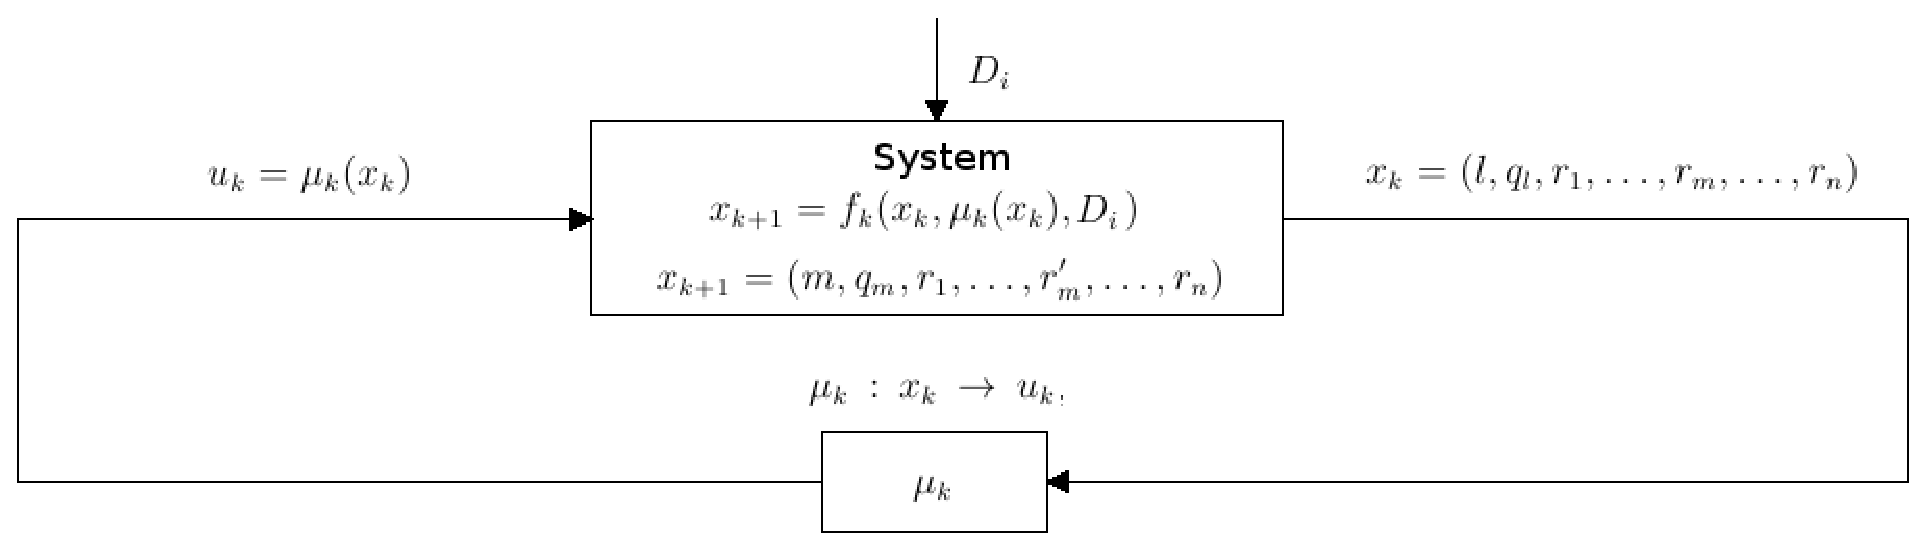
\includegraphics[width=1\textwidth]{Images/Chapter2/System_SDP.eps}
  \end{center}
    \caption{Stochastic Dynamic System for VRPSD}\label{fig:SDPS_VRPSD}
\end{figure}

Incurring in a transition cost $g(x_k,u_k,x_{k+1})$

\begin{equation}\label{eq:costg}
    g(x_k,\mu_k(x_k),x_{k+1}) = \left \{ \begin{array}{ll}
    d(l,m), & \text{whether } u_k(m,0)=\mu_k(x_k)\\
    d(l,0) + d(0,m), & \text{whether } u_k(m,1)=\mu_k(x_k)
    \end{array} \right.
 \end{equation}

The objective of the problem is to find a policy $\pi$ that minimizes the cost of transport $J_N^\pi$ (\ref{eq:SDP_obj_VRPSD}) in the $N$-stages or the expected cost to complete given an initial state. The optimal cost of transport in the $N$-stage $x$ is  $J_N^*(x) = min_{\pi\in \Pi}J_N^\pi(x)$, where $\Pi$ is the set of admissible policies. 

\begin{equation}\label{eq:SDP_obj_VRPSD}
 J_N^\pi(x_0)=E\biggr\{\sum_{k=0}^{N-1}g(x_k,\mu_k(x_k),x_{k+1})\biggr\}
\end{equation}

If $J_N^*(x)$ is known for all stages, the optimal control $u_k^*$ at each stage is to find the minimum of the following equation (\ref{eq:u_k^*}):

\begin{multline}\label{eq:u_k^*}
     u_k^*=\mu_k^*(x)=
\arg\min\limits_{u_k \in U_k(x_k)}g(x_k,u_k,x_{k+1})+\\
\sum_{x_{k+1}\in S}p_{x_kx_{k+1}}(u_k)J_N^*(x_{k+1})|x_k=x, \forall x\in S
\end{multline}

The problem is that $J_N^*(x)$ is unknown and its calculation is a computationally intractable problem given the size of state space. Secomandi ~\cite{secomandi_rollout_2001} points out that computing an optimal policy becomes quickly intractable when $n$ grows beyond 10. Chapter \ref{chap:dp_methodology} deals with issue of approximating this function through a dynamic-programming method efficiently computable.

\section{Summary}

The VRPSD has been studied for more than 20 years, with important progress in 90's and 00's and wide areas of application in logistics, following the conclusions of ~\cite{Dror_2005} the most promising approach is modeling the problem as a Markov decision process. Hence, a stochastic programming model is selected: a methodology for sequential decisions made under uncertainty, based on dynamic system, where the main idea is to use an approximate a function $J$ in order to make decisions in complex dynamic systems, allowing to deal with instances considered intractable for their size. In the next section, the dynamic programming solution is addressed.

%////////////////////////////////////////////////////////////////////////////////////////////////////////////////////////////////////////////////
%Stochastic dynamic programming
 \chapter{Stochastic Dynamic programming solution}
\label{chap:dp_methodology}
%\minitoc


\section{Dynamic approach for VRPSD}

Dynamic programming is based on principle of optimality formuled by Bellman ~\cite{bellman_theory_1954}

\begin{quote}
 \textit{An optimal policy has the property that whatever the initial state and initial decision are, the remaining decisions must constitute an optimal policy with regard to the state resulting from the first decision.}
\end{quote}

Following to Bertsekas ~\cite{bertsekas_dynamic_1995} the principle of optimality point out that an optimal policy can be constructed backward, first finding an optimal policy for the \textit{tail subproblem} involving the last stage, then extending the optimal policy to the problem regard with the last two stages, and continuing until cover the whole problem in the first stage, hence a optimal policy is constructed for the entire problem.

\begin{multline}
 J^*(x_0) = \min\limits_{u_k^*\in U_k(x_k)}E_{w_k}\biggr\{g_k(x_k,u_k^*,w_k)+J^*_{k+1}(f(x_k,u_k^*,w_k))\biggr\},\\
\forall k=0,1,\ldots,N-1
\end{multline}

However, the exact assesing of $J^*$ is computationally infeasible given the size of the state space. Therefore, is necessary approximate it function for generate good, but not necessarily optimal policies.

Let $\tilde{J}_k$ be an approximation of $J^*_k$, then a control can $\tilde{u}_k$ be assesed

\begin{equation}\label{eq:control_aprox}
\tilde{u}_k=\tilde{\mu}_k(x_k)=\arg \min\limits_{u\in U_k(x_k)} \biggr\{ g(x_k,u_k,x_{k+1}) + \sum_{x_{k+1}\in S}p_{x_kx_{k+1}}\biggr\}
\end{equation}

The following section \ref{sec:expecteddistance} discuss the computation of $\tilde{J}_k$

\subsection{Expected distance}\label{sec:expecteddistance}

The expected distance $\tilde{J}$ or \textit{cost-to-go} is computed based on the algorithm propossed by Secomandi ~\cite{secomandi_rollout_2001}. We implemented the algorithm $\Gamma$ represented below \ref{algo:expecteddistance} to compute expected distance in $O(nRQ)$ time and $O(nQ)$ space.

\begin{algorithm}
\SetKwInOut{Input}{input}\SetKwInOut{Output}{output}
 \Input{tour $\tau_{1\times n+2}$, $d_{n+1\times n+1}$ distance, $x$ state}
\Output{$E$ expected distance of an apriori solution $\tau$ (base sequence)}
$l = x_1$\;
$q_l = x_2$\;
\If(is the last customer on $\tau$){ $l = n$ }{%if l == tau(instance.n+1)
  $E = d(\tau(l+1)+1,1)$\;%d(n,0)
}
\Else{
  \If(is the first node \textit{depot} in the tour $\tau$){l=0}{
    E = $\Gamma ( \tau, l+1, q_l)$\;
  }
  \Else{
    $E_0 = d(\tau(l+1), \tau(l))+$%\;%d(i+1,i)    
    $\sum_{j=0}^{\min\{q_l, \bar{D}_{\tau(l+1)}\}}\Gamma(\tau,l+1,q_l-j)*p^{\tau(l+1)}(j) +$%\;
    $\sum_{j=q_l+1}^{\bar{D}_{\tau(l+1)}}2 * d(0,\tau(l+1))+ %d(0,i+1)
                \Gamma(\tau,l+1,Q + q_l-j))*p^{\tau(l+1)}(j)$\;
    %
    $E_1 = d(0,\tau(l)) + d(0, \tau(l+1)) + $%\;%d(0,i)+d(0,i+1)
    $\sum_{j=0}^{\bar{D}(\tau(l+1))} \Gamma(\tau,l+1,Q-j)*p^{\tau(l+1)}(j)$\;
    $E=\min\{E_0,E_1\}$\;
  }  
}

\caption{Expected distance algorithm $E = \Gamma(\tau,l,q_i)$}\label{algo:expecteddistance}
\end{algorithm}

This algorithm was validated comparing the outcomes with the expected distance computed by an exhaustive algorithm applied to small instances. In addition, larger instances was benchmarked using monte carlo simulation to asses expected distance.

If the vehicle capacity is depleted, the methods used to compute the expected distance take into account that the vehicle can go to the depot for proactive restocking with less cost than to visit the customer first which makes the route fail, as we show in \ref{th:proactive_restocking}.

\begin{theorem}\label{th:proactive_restocking}%check redaction
 if $q_l=0$ then the vehicle must go first to the depot for replenishment and later visit the next customer on the route, it is better than it visit the next customer to know its demand and go to the depot for replanishment after.
\end{theorem}

\begin{proof}
Given the current state $x_k=(l,0,r_1,\ldots, r_n)$ where the vehicle capacity is depleted, i.e. $q_l = 0$, assume that the next customer to be visited on the route is $l'$. If the customer is visited first, then the vehicle must go to depot for replenishment and go back to $l'$ to satisfy its demand, so the distance is $\delta(l,l')+2\delta(l',0)$. Otherwise, if a proactive restocking of the vehicle is performed then the total distance is $\delta(l,0)+\delta(0,l')$.
Assume $\delta(l,0)+\delta(0,l') \leq \delta(l,l')+2\delta(l',0)$ then by triangular inequality $\delta(l,0) \leq \delta(l,l')+\delta(l',0)$ proving \ref{th:proactive_restocking}
\end{proof}

\begin{lemma}%chech redaction
 The theorem \ref{th:proactive_restocking} can be generalized for all $q_l \geq D_i'$ where $D_i'$ is the demand of the customer $i$ who is the next on the tour.
\end{lemma}






%\section{Probabilistic policy}

%Use probability distribution to determine the apriori tour $\tau$ which should be followed

%1- Is possible use un TSP solution method and combine with probability distribution function.

%2- Heuristic based on distance and probabilities

%3- Greedy algorithm with probabilities information to define replanishments

\section{Policy iteration}

The policy iteration algorithm is a dynamic programming technnique, it generates a sequence of stationary policies, each with improved cost over the preceding one. The algorithm describe the following sequence of steps \ref{algo:policy_iteration_general}:

\begin{algorithm}
 \textbf{1. Initialization:} Guess an initial stationary policy $\pi_0$\\
 \textbf{2. Policy evaluation:} Given the stationary policy $\pi_k$ compute the corresponding cost function $J_{\pi_k}$\\
 \textbf{3. Policy improvement:} Obtain a new stationary policy $\pi_{k+1}$\\
 Repeat step 2 to 3\\
 \caption{Policy iteration algorithm}\label{algo:policy_iteration_general}
\end{algorithm}

If the policy evaluation step compute $J_{\pi_k}(x)$ for all states $x \in S$ and the algorithm runs until  $J_{\pi_m} = J_{\pi_{m+1}}$, $\forall x \in S$ then the algorithm finds the optimal policy $\pi^*$. In contrast, when $|S|$ is too large this algorithm is inpractical; although these steps can be approximated to deal with large-scale systems despite that convergence to optimal solution is not guaranteed.


\subsection{Rollout algorithm}
%\subsection{One-step rollout algorithm}

The rollout algorithm is an approximate policy iteration technnique, used to to increase the effectiveness of a heuristic by iteratively applying it, or rolling it out, at each decision stage (Goodson, 2010). The algorithm require to know a base policy $\pi$ for the problem. Also assume that the cost-to-go of this base policy from any given state $x$ can be easily computed (Secomandi, 2000). Thus, it build a policy $\pi$ starting from any given state and following an \textit{a priori} solution to VRPSD.


\subsubsection{Defining initial policy}\label{sec:initial_policy}


Cyclic heuristic $\mathcal{C}$ shifts $\tau$ to obtain an permutation keeping an cyclic order. It builds the cyclic tour that start at $l$ and follow $\tau$ cyclically, so, $\tau^\mathcal{C}_l = (l, l+1, \ldots , n , 1 , \ldots , l-1, 0)$ represent an apriori policy $\pi^\mathcal{C}$. Cyclic heuristic was propossed by Bertsimas 92  and improved by himsel 95 and later used by a many authors because it is simple, inexpensive and sequentially consistent (Secomandi dissertation, 1998)

Following cyclic heuristic the rollout algorithm \ref{algo:rollout} describe a fixed number of iterations given an instance of the problem changing $\tau$ after the first state. Since there are a transition of $x_l$ state to $x_{l+1}$, is only shifted the segment of $\tau$ that follow to $l$, maintaining in this section the customers still no visited or with demand different to $0$. Since that already fully served customers are assumed to be skipped in $\tau^\mathcal{C}_l$.

%(Solution alternatives for following \tau in rollout algorithm)
%This is a topic that must be discussed with the group
%Option 1 


%Option 2
In order to compute rollout policy controls, the control which define the first customer $l_1$ to be visited by $\tilde{\pi}^\mathcal{C}$ is found as:

\[\mu_0(x_0) = u_0 = (l_1,0) = \arg\min\limits_{l \in V-\{0\}} \{\tilde{J}_{\pi_0}(x_0)\}\]

where the expected length $\tilde{J}_{\pi_0}(x_0)$ of ${\pi_0}$ which follow the cylcic tour $\tau^\mathcal{C}_l=(0,l,l+1,\ldots,1,n,\ldots,l-1,0)$, in the initial state $x_0$, is computed using the algorithm $\Gamma$ \ref{algo:expecteddistance}. Hence, the system moves to next state visiting the customer $l_1$ directrly who is fully served since $q_0 = Q$ and $r_l \leq Q$.


 
\begin{algorithm}
\SetKwInOut{Input}{input}\SetKwInOut{Output}{output}
\SetKwRepeat{Repeat}{repeat}{until}
\Input{$\pi_0$, state $x_0$}
\Output{$\tilde{\pi}^\mathcal{C}$ policy} 
Given a initial policy $\pi_0=u_1,u_2,\ldots u_{N-1}$ and initial state $x_0$ \\
$\tilde{\pi}^\mathcal{C} = \emptyset$\\
\Repeat{the final state $x_N$ is reached}{
$\tilde{\mu_k} = \arg\min\limits_{u_k \in U_k(x_k)} \{\min\{\tilde{J}^0_{\pi_k}(x_k),\tilde{J}^1_{\pi_k}(x_k)\}\}$\\
Add $\tilde{\mu_k}$ to $\tilde{\pi}^\mathcal{C}$\\
Apply the control $\tilde{\mu_k}$ to the state $x_k$.i.e.
$x_{k+1} = f_k(x_k,\tilde{\mu_k}(x_k),D)$\\
Roll out $\pi_k$ since $\tilde{\mu_k}$ to $\mu_{N-1}$ following cyclic heuristic\\
}
\caption{Rollout algorithm}\label{algo:rollout}
\end{algorithm}


For some state $x_k = (k,q_k,r_1,\ldots,r_n)$, $\tilde{J}^0_{\pi_k}(x_k)$ compute the expected distance of move the vehicle directly to the next customer following the policy ${\pi_k}$ thereafter.

\begin{equation}\label{ra:Cost2Go0}%Review notation
 \tilde{J}^0_{\pi_k}(x_k)=d(\tau_l,m)+\sum_{k=0}^{q_l}p_m(k)\Gamma(\tau,l+1,q_l-k)+\sum_{k=q_l+1}^{K_m}2d(0,m)p_m(k)\Gamma(\tau,l+1,q_l+Q-k)%Review if \Gamma(\tau,l+1,q_l+Q-k) or \Gamma(\tau,l+1,Q-k)
\end{equation}

While $\tilde{J}^1_{\pi_k}(x_k)$ assess the expected distance performing an proactive replanishment before of move the vehicle to the next customer following the policy ${\pi_k}$ thereafter.

\begin{equation}\label{ra:Cost2Go1}%Review notation
 \tilde{J}^1_{\pi_k}(x_k)=d(0,\tau_l)+d(0,m)+\sum_{k=0}^{K_m}p_m(k)\Gamma(\tau,l+1,Q-k)
\end{equation}

Thus, the control $\tilde{\mu_k}$ which decides to visit the customer $l$ is computed as follows depending on the smaller cost:

\begin{equation}\label{eq:costg}
    \tilde{\mu_k} = \left \{ \begin{array}{ll}
    (l,0), & \text{if } \tilde{J}^0_{\pi_k}(x_k) \leq \tilde{J}^1_{\pi_k}(x_k)\\
    (l,1), & \text{in other case}
    \end{array} \right.
 \end{equation}


%complexity

Rollout explore $\frac{1}{2}n(n+1)$ different policies with an computational cost of $O(nRQ)$ in order to evaluate the expected distance for each one, hence, the rollout algorithm runs in $O(n^3RQ)$ time.

% \subsubsection{Partial rollout algorithm}

\section{Summary}

Rollout algorithm is an approximate atochastic dynamic programming technnique implemented to improve a \textit{a priori} policy. We use cyclic heuristic as base policy since it is simple, inexpensive and sequentially consistent. Finally. we describe the rollout algorithm and point out the computational complexity to perform it.






%////////////////////////////////////////////////////////////////////////////////////////////////////////////////////////////////////////////////
%hybrid GA
 \chapter{Hybrid evolutionary approach}
\label{chap:methodology}
%\minitoc

An evolutionary algorithm is a technique bio-inspired by the evolution of the espicies. It was proposed by John Holland early in the 70's (Holland, 1975). This algorithm seeks to evolve a population of individuals that represent solutions to the problem through genetic operators such as crossover, mutations and selection. The population generated in each iteration is evaluated and then the individuals with a better fitness are chosen for the next generation with more chance.

\section{Hybrid genetic algorithm}

A hybrid evolutionary algorithms or hybrid genetic algorithms are a very popular techniques that offers practical advantages to deal with complex and hardly optimization problems. Grosan (Grosan, 2007) present a review of hybrid genetic architectures frecuently used. 

Hybridization can be performed using prior knowledge, heuristics, local search, other techniques. We use it to carry out local search through rollout algorithm. Some times, a hybrid genetic algorithm which combine other technique to local search is known as memetic algorithm.

Generally, the purpose of hibridization is:

\begin{itemize}
 \item Improve the performance of the evolutionary algorithms.
 \item Improve quality of solutions obtained by evolutionary algorithm
 \item Incorporate evolutionary algorithm as part of a large system
\end{itemize}

Evolutionary algorithm behavior is determined by the exploitation and exploration; In exploitation local search is performed to improve solutions, and exploration avoid local optimum extending the search space, our implementation of memetic algorithm works to keep these relation throughout the run. So, in this application hybridazation not only improve the quality of the solutions obtained by evolutionary algorithm, also is assembly as an framework for rollout algorithm in order to avoid local optimum.


\subsection{A basic genetic algorithm for vehicle routing problem with stochastic demands}

We show an example of basic GA in general form in figure \ref{fig:ga_basic}. First, an initial population is selected and fitness function is assessed for each individual in the population. In order to produce a new population for the next generation, crossover and mutation operators are applied to individuals allowing those who have better fitness function to get more chances to reproduce themselves. In the selection stage, offspring's fitness is evaluated to choose the individuals to integrate the new population; individuals with competitive fitness regarding to the population have more probability to be selected. These steps are repeated until stopping criteriums are resolve.

\begin{figure}[!htbp]
  \begin{center}
   \includegraphics[width=0.6\textwidth]{Images/Chapter3/ga_basic.eps}
  \end{center}
    \caption{Basic genetic algorithm}\label{fig:ga_basic}
\end{figure}

\subsubsection*{Initialization}

We represent an individual in the population as a policy tour $\pi^\mathcal{C}$ whose fitness is the expected distance $\tilde{J}_{\pi^\mathcal{C}}$ computed using the algorithm $\Gamma$ \ref{algo:expecteddistance}.

The initial population $P_0$ with an fixed size $|P_0| = n$, is obtained using the cyclic heuristic in $O(n)$ time. It performs in order to reduce the computational cost since we can evaluate fitness to $P_0$ in $O(n)$ time when rollout is accomplished under some individual in the population.


\subsubsection*{Crossover}

The crossover operator $\circledast$ consist in to select two different individuals $I^{P_k}_i$ and $I^{P_k}_j$ with probability dependently of their fitness value respectively; meanwhile, a random cut point $\rho \in [1,n]$ is selected uniformly. So, a new individual raise to concatenate the subsequence $I^{P_k}_i[1..\rho]$ with the subsequence $I^{P_k}_j[\rho+1,..,n]$. 

A crossover operation can yield an new individual that represents an unfeasible policy. However, we implement this operator to run in time $O(n^2)$ and guaraneeing only feasible solutions as a result.


\subsubsection*{Mutation}

This operator performs three types of mutation with same probability to produce and individual in the offspring: swap two elements of policy selected randomly, flip a random subsequence of policy or shift the policy an random number of times.

The mutation of an individual can happened with probability $Prob_m = 0.04$ in the experiments presented in this document and it compute in $O(1)$ time.


\subsubsection*{Selection of the new population}

New population originates as a result of crossover and mutation operators. However, the evolutionary algorithm also obtain individuals to the offspring performing the cyclic heuristic. Hence, those who have better fitness can be choosen with more chance to integrate the new population.

In order to punish generation which dicrease the fitness and reward to those who increase this value respect to the previos generation the size or number of individuals available to the next generation changes.

Let $\Delta^{P_k}_{E'}$ be the rate of fitness change in the generation $P_k$, i.e.

\begin{equation}\label{eq:improve_fitness}
 \Delta^{P_k}_{E'} = \frac{\bar{\Gamma}_{P_{k-1}} - \bar{\Gamma}_{P_k}}{\bar{\Gamma}_{P_{k-1}}} 
\end{equation}

where $\bar{\Gamma}_{P_k}$ is the best expected distance obtained by an individual in the generation $k$.

Then, the size of the next population $P_{k+1}$ is computed so:

\begin{equation}\label{eq:population_size}
 ||P_{k+1}|| = \left \{ \begin{array}{ll}
  \lfloor  \min\{n(1+\alpha), ||P_{k}||(1+\alpha)\} \rfloor, & \text{if } \Delta^{P_k}_{E'} > 0\\
  \lceil \max\{n\alpha, ||P_{k}||\alpha\} \rceil, & \text{if } \Delta^{P_k}_{E'} < 0
  ||P_{k}||, \text{in other case.}
  \end{array} \right.
\end{equation}


where $\alpha$ is a tuneable parameter which should be fixed in the range $(0,1]$ depending of computational resources. Consequently it reward a offspring that improve the quality of the solutions in comparison to theirs parents, increasing the population size at most an $\alpha$ times the size. Otherwise, when the quality of the solutions decrease respect to the previos generation, the size of population is punished decreasing it at least an $\alpha$ factor of the size of population. The figure \ref{fig:ga_basic_i_30r1} shows results of basic genetic algorithm applied to one instance with $\alpha = 0.5$, the last chart below on the right side of figure exhibit the size of population for each generation.

\begin{figure}[!htbp]
  \begin{center}
   \includegraphics[width=0.9\textwidth]{Images/Chapter3/i_30r1_regular.eps}
  \end{center}
    \caption{Basic genetic algorithm applied to instance of 30 customers. The second image in the first row ilustrate the last population and the next image shows the best solution finded. }\label{fig:ga_basic_i_30r1}
\end{figure}

\subsubsection*{Stopping criterion}

Finally, the evolutionary algorithm runs until reach a fixed number or iterations $\kappa$. Nevertheless, it can stop once accopmlish $\mathbf{m}$ number of consecutive iterations whitous a significative change, i.e., $|\Delta^{P_k}_{E'}|\leq \varepsilon$

% \subsubsection{Crossover - EAX}

% Edge assembly crossover

% \subsubsection*{Mutation}

% Swap

\subsubsection*{local search}


A classic genetic algorithm does not yield competitive results itself, due to simple GA does not exploit problem knowing to produce high quality solutions. To be effective, we combine local search methods.


Often hybridazation is included in inicialization and reproduction operators.

local search can be incorporated in the initial population or among the offspring.

\subsubsection*{Performance of the genetic algorithms}

This section describes the algorithm performance for a specific problem instance with 10 customers and a factor $f'=1$, the customers' location and demand value (known when the vehicle arrive to the customer location) are showed in the figure \ref{fig:customer_n10_f1_s1}.


%\begin{figure}[!htbp]
%  \begin{center}
%    \includegraphics[width=0.9\textwidth]{Chapitre3/n10_f1_s1_customers}
%  \end{center}
%    \caption{Instance features: $n = 10$, $seed = 1$, $f' = 1$}\label{fig:customer_n10_f1_s1}
%\end{figure}

The genetic algorithm outcome for the instance problem described above is presented in the figure \ref{fig:tour_n10_f1_s1}, the red line describes the route, the segmented black line represents returns to the depot for replenishment, this tour was selected as the best solution found in 100 iterations of the GA.

%\begin{figure}[!htbp]
%  \begin{center}
%    \includegraphics[width=0.9\textwidth]{Chapitre3/n10_f1_s1_tour}
%  \end{center}
%      \caption{e.g best tour found by the GA: $n = 10$, $seed = 1$, $f' = 1$}\label{fig:tour_n10_f1_s1}
%\end{figure}

The figure \ref{fig:improve_n10_f1_s1} shows the improving of the objective function found, the chart shows the lesser total cost history, when a better value is found the line fall, therefore we can see the improving is given among the iteration 25 and 40, after this iterations the algorithm converges and it's not found a better solution.

%\begin{figure}[!htbp]
%  \begin{center}
%    \includegraphics[width=0.9\textwidth]{Chapitre3/n10_f1_s1_history}
%  \end{center}
%      \caption{e.g improvement solution: $n = 10$, $seed = 1$, $f' = 1$}\label{fig:improve_n10_f1_s1}
%\end{figure}

%\section{Memetic Algorithm}

%GA that use local search

%\section{Non-dominated Genetic Algorithm}


%////////////////////////////////////////////////////////////////////////////////////////////////////////////////////////////////////////////////

%Results
 \chapter{Experiments and Numerical Results}
\label{chap:results}
%\minitoc

\section{Instances of VRPSD}

To compare results we are used instances of two diferents sources, the first set of instances was generated following a procedure similar to the used in Secomandi~\cite{secomandi_comparing_2000}, the another set of instances is the used by Novoa ~\cite{novoa_approximate_2009}, Both instance sets are generated using the procedure described on the next section.

\subsection{Instance generation}

The set of instances contain 45 different instances resulting from combine three number of customers $n \in \{5,10,20\}$, three vehicle capacities given for $f'$ factor and five different assignments for customer locations and demand distribution for each one, the assignments result from changing the random seeds.

The customers' demands are both discrete and distributed uniformly in this posible sets $U[1,5]$, $U[3,9]$, $U[6,12]$, in each instance, each customer is assigned to any of the three groups with equal probability. Customers' locations are random points in $[0, 1]^2$, with the depot fixed at $(0,0)$.%, e.g. figure \ref{fig:instance_n5_f1_s1}.

%\begin{figure}[h]
  % Requires \usepackage{graphicx}
%  \includegraphics[scale=0.4]{images/n5_f1_s1}\\
%  \caption{Customers' location, n = 5}\label{fig:instance_n5_f1_s1}
%\end{figure}

The filling rate $f$ is an index of the total expected demand relative to vehicle capacity.

\begin{equation}\label{eq:4filling-rate}
f=\sum_{i=1}^n\frac{E[D_i]}{mQ}
\end{equation}

where $E[D_i]$ is the expected demand of customer $i$, $m$ is the number of available vehicles, when $m = 1$ $f$ can represent approximately the expected number of replenishment needed to serve all customers' demands. It follows that, a priori, in all instances $E[D_i]=(3+6+9)/3=6$, for any customer i, and $Q=6n/f$. $f'=f-1$ is the expected number of route failure in a given instance. Hence, we is defined for this factor $f' \in \{1.0, 1.5, 2.0\}$, following the same factors used by Secomandi~\cite{secomandi_comparing_2000}.

\begin{table}
  \centering
  \caption{Vehicle capacity for each factor}\label{tb:Q}
\begin{tabular}{l l l l}
  \hline
  % after \\: \hline or \cline{col1-col2} \cline{col3-col4} ...
  $f'$ &   & $n$ &   \\
  \cline{2-4}
      & 5 & 10 & 15 \\
  \hline
  1.0 & 15 & 30 & 45 \\
  1.5 & 12 & 24 & 36 \\
  2.0 & 10 & 20 & 30 \\
  \hline
\end{tabular}
\end{table}

The 160 instances used by Novoa ~\cite{novoa_approximate_2009} are composed by 70 small size instances (5 to 20 vertex), 60 medium size (30 to 60 vertex) and 30 instances of large size whose number of vertex is greter than 100.

\section{Assess the expected distance for a given policy}

straightforward policy is better than cyclic policy at each one instance tested \ref{fig:avg_distance_cyclic_vs_avg_distance_forward}

\begin{figure}[!htbp]
  \begin{center}
   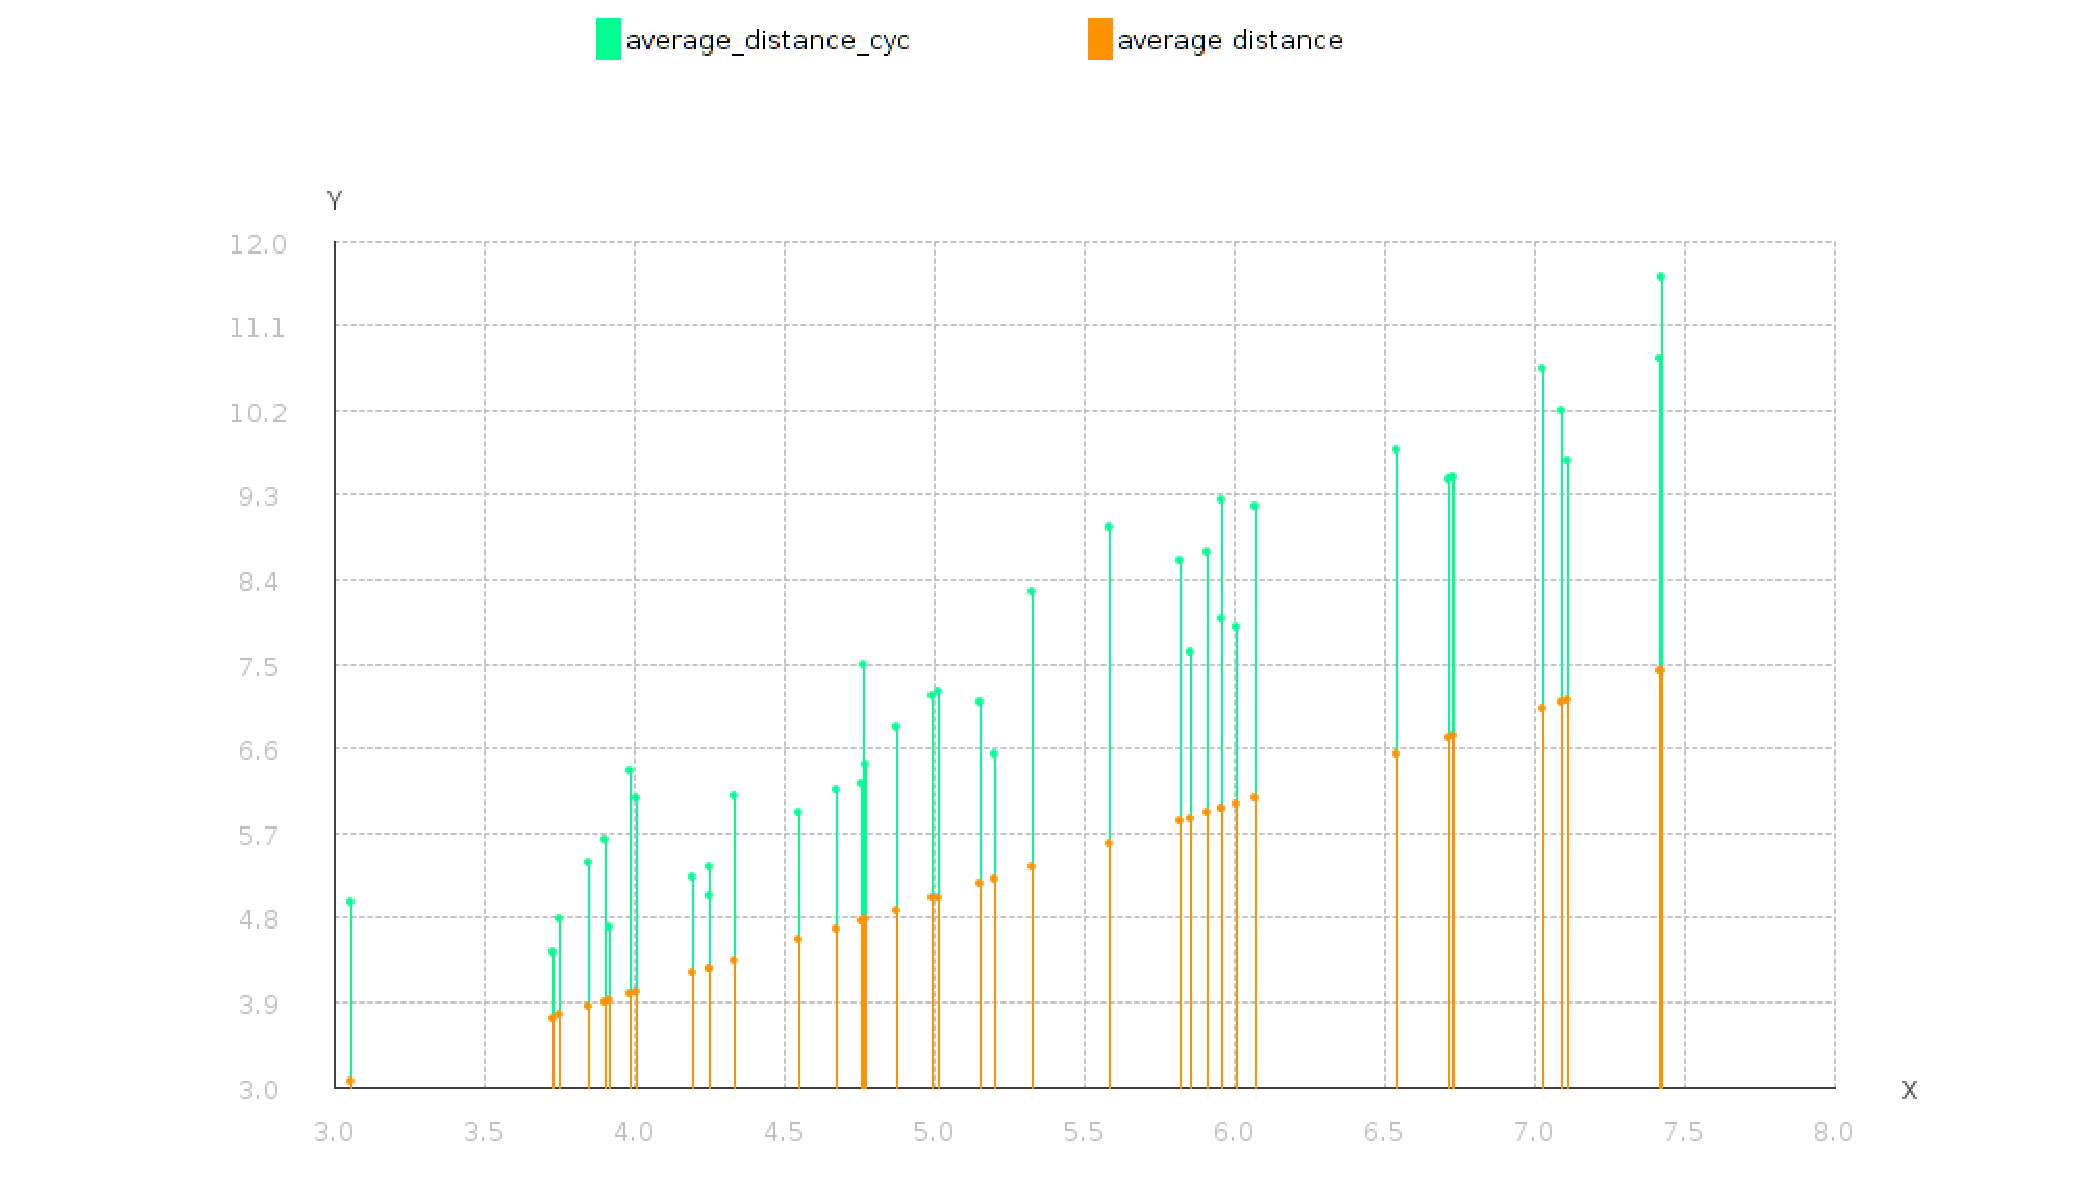
\includegraphics[width=1\textwidth]{Images/Chapter5/cyclic_vs_straightforward_avgdistance_n5_n8.eps}
  \end{center}
    \caption{average distance straightforward tour vs. average distance cyclic tour}\label{fig:avg_distance_cyclic_vs_avg_distance_forward}
\end{figure}

\subsection{Expected distance algorithm}\label{sec:test_expecteddistance}

Validation of backward expected distance algorithm comparing with the average expected distance of a tour $\tau$, where $\tau$ is assumed as a sorted permutation of the nodes, i.e. $\tau = (1,\ldots,n,0)$. The average expected distance is computed using monte carlo simulation under policy $\pi$ following $\tau$ and considering early replenishments defined by the policy.

\begin{figure}[!htbp]
  \begin{center}
   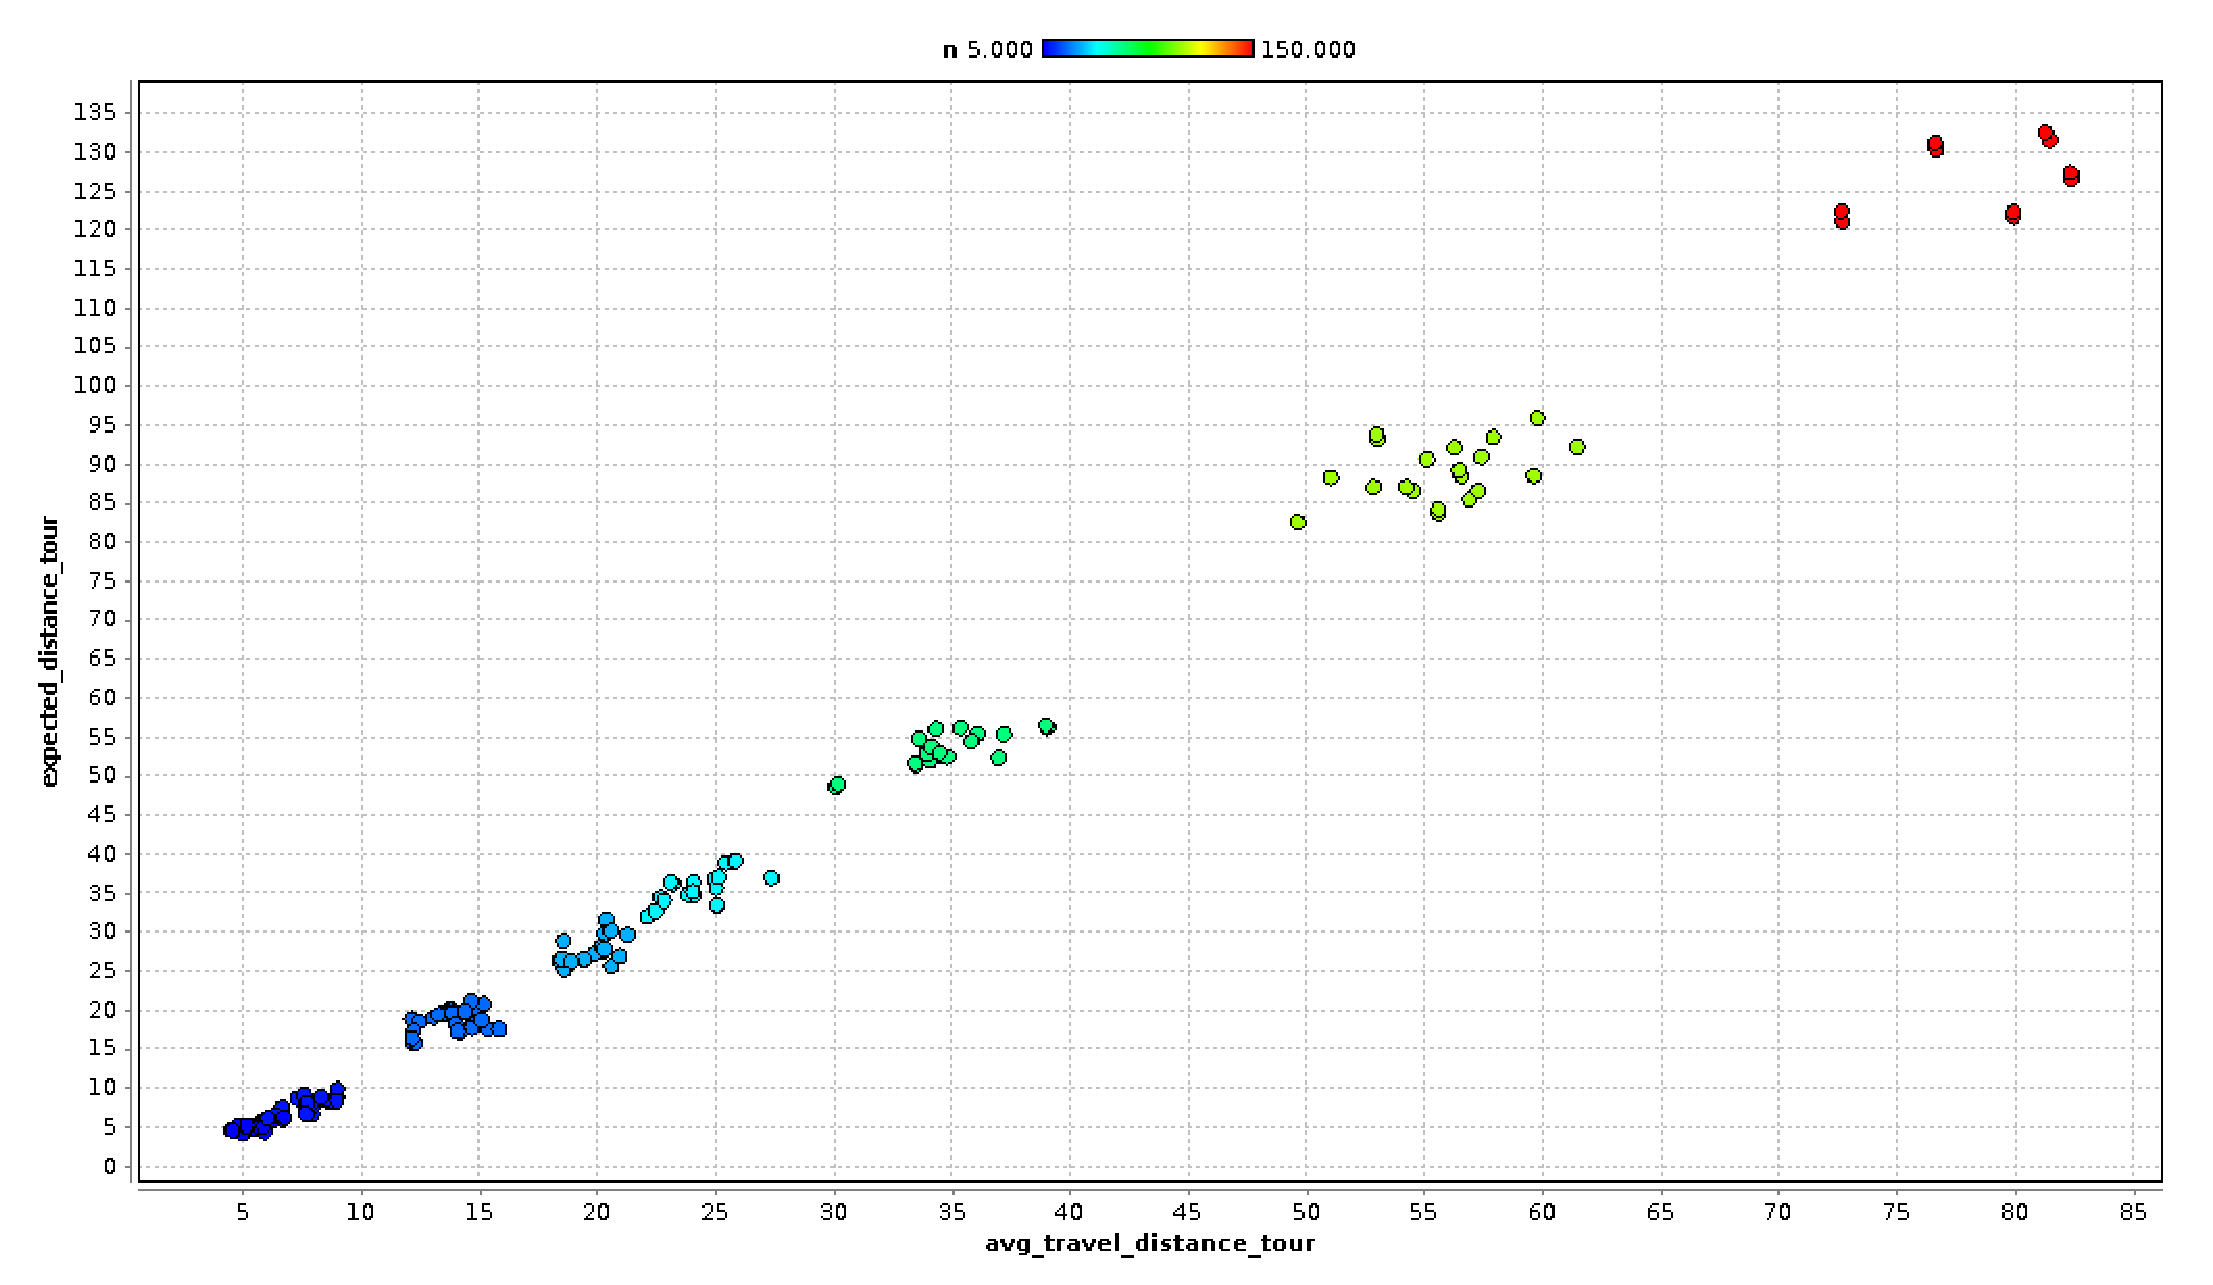
\includegraphics[width=1\textwidth]{Images/Chapter5/avg_vs_expected_distance_tour.eps}
  \end{center}
    \caption{average distance tour vs. expected distance tour}\label{fig:avg_distance_vs_expected_distance_tour}
\end{figure}

\begin{figure}[!htbp]
  \begin{center}
   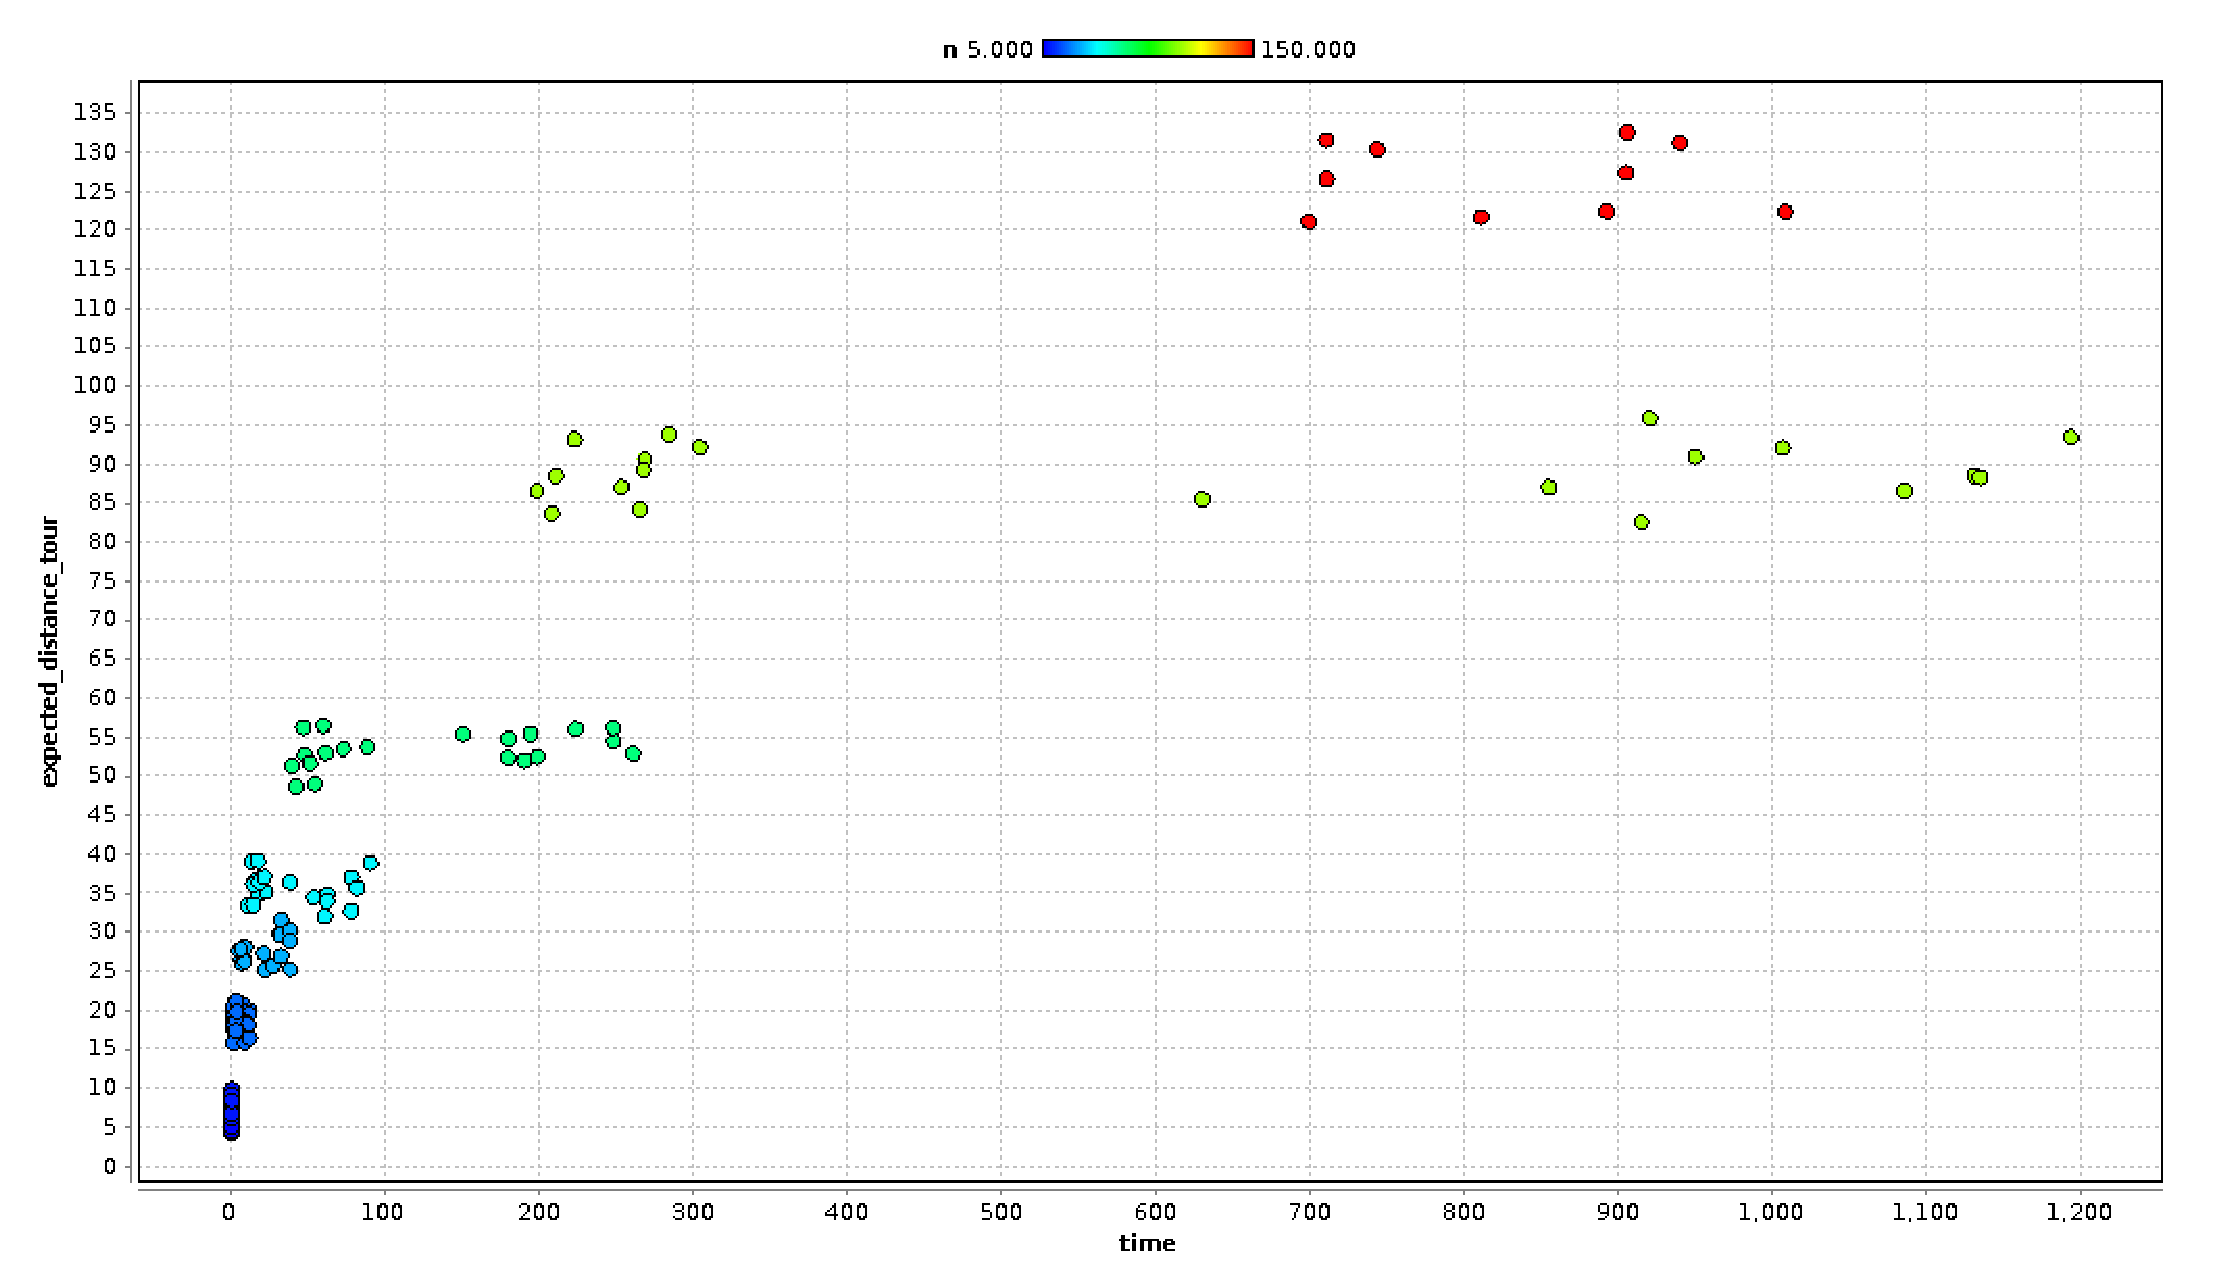
\includegraphics[width=1\textwidth]{Images/Chapter5/time_vs_expected_distance_tour.eps}
  \end{center}
    \caption{execution algorithm time vs. expected distance tour}\label{fig:time_distance_vs_expected_distance_tour}
\end{figure}

%Discussion of results, conclussion and future works
 \chapter{Conclusions}
\label{chap:conclusions}
%\minitoc


Although the hybridization approach increases the computational time cost, this effort is rewarded in many cases given that the quality of the solutions is improved than if we apply the rollout algorithm alone. 

Hence, since the local searchis performed every time a new solution is generated.

Often memetic algorithms employ long runnig times because local search is the most time-consuming component. For this reason, we partialy apply the rollout algorithm in large instances to reduce the time consumption to compute the solution.

Although the genetic operators attempt to explore by extending the search space to avoid local optimum. This operators by themselves do not improve the solutions. So, it is necessary to focus on local search to improve the quality solutions and the convergence.

To evaluate expected distance consume a lot of computational time, so an efficient approximation improves the algorithm performance.

Given that local search is performed every time a new solution si generated often memetic algorithms employ long runnig times. 

Local search is the most time-consuming component.

Evaluate expected distance consume a lot of execution time, efficiently approximation improve the algorithm performance.

Focus local search improve the quality solutions and the convergency.

when local search is applied the evolutionary algorithm stops when the number of iterations is achived.

In the behavior of the genetic algorithms with small and medium instances, we observe that if local search is applied the evolutionary algorithm stops when the number of iterations is achived, rather than basic genetic algorithm where often complete the maximun counting of iterations without significative change. This can be observed in the figure \ref{fig:ga_basic_mvi_20r4_m} in comparison with the figure \ref{fig:memetic_mvi_20r4_m}. We expected that local search accelerate the convergence of solution in the memetic algorithm.

In spite of that basic genetic algorithm often expend less time, the hybrid approach finds a solution employing less time for many large instances. Memetic algorithm can perform less iterations since obtain an unbeatable solution early inducing the algorithm to stop to accomplish the number of iterations whitout significative change. %this contradice 


when instance size increase also grow the distance between the quality of solutions finded by memetic algorithm and the solutions computed by others.

Not only memetic algorithm obtained better results than others algorithms implemented, also its outcomes have less variability

ra is inexpensive

memetic consume similar running time in large instances than basic genetic algorithm but it obtain better results.

genetic algorithm is more inexpensive than memetic in small and medium instances

ra is better than basic genetic since it obtain better results employing less computational resources.




\section*{Perspectives}


 %Appendixes
 %Appendix 1: Algorithms detailed
 \begin{appendix}
\chapter{Algorithms}
\label{chap:appendix1}

\section{Algorithms detaileds}



\begin{algorithm}

\SetKwInOut{Input}{input}\SetKwInOut{Output}{output}
 \Input{tour $\tau_{1\times n+2}$, state $x_{1 \times n+2}$}
\Output{$\pi$ policy}
$\bar\tau = \tau$\;
$i=1$\;
\While{$x \neq x_f$}{
$\tau = \bar\tau$\;
  \For{$j \in SN$}{
    \If(is the first node in the tour $\tau$, i.e. l=0){i=1}{
      $\tilde{J} = \Gamma(\tau,0,q_l)$\;
      $a_{min} = 0$\;
    }
    \Else{%General case
      $J^0 = g^0(i, \tau_{i+1}, x)$\;
      $J^1 = g^1(i, \tau_{i+1}, x)$\;
      $\tilde{J} = \min\{J^0,J^1\}$\;
      $a = \arg\min\{J^0,J^1\} - 1$\;
    }
    %Evaluate minimization
    \If{$\tilde{J}_{min} > \tilde{J}$}{
      $\tilde{J}_{min} = \tilde{J}$\;
      $a_{min} = a$\;
      $\bar\tau = \tau$\;
      $\tau = sh(\tau,i)$\;
    }
  }
  $l=\bar\tau_{i+1}$\;
  $\pi\leftarrow u=(l,a_{min})$\;
  $x=\Upsilon(x,u)$\;
  \If{$r_l=0$}{
    $SN = SN-l$\;
  }
  $i=i+1$\;
}
\caption{Rollout algorithm}\label{algo:rollout1step}
\end{algorithm}

where SN is the set of nodes that still need to be visited, i.e. $\forall l \in N, D_l > 0$, 
$x_f$ is the final state, where the vehicle comeback to depot and each customer was visited and its demand is $0$, $x=(0,Q,0,\ldots,0)$, $\bar\tau$ is the minimum $\tau$ selected in each algorithm iteration.
$q_l = x_2$, $l=x_1$ and $r_l=x_{l+2}$\\
When $l=0$ or $i=1$ in the algorithm, $q_l = Q$
$sh(\tau,i)$ shift sub $\tau$ vector from position $i$ to the final position. 

The $g^a(l,m,x)$ function is the expected distance from $l$ to $m$ given the state $x$, where $a=1$ if earlier replanishment is specified or $a=0$ in otherwise. The function is described below.
\begin{equation}\label{ra:Cost2Go0}
 g^0(l,m,x)=d(\tau_l,m)+\sum_{k=0}^{q_l}p_m(k)\Gamma(\tau,l+1,q_l-k)+\sum_{k=q_l+1}^{K_m}2d(0,m)p_m(k)\Gamma(\tau,l+1,q_l+Q-k)%Review if \Gamma(\tau,l+1,q_l+Q-k) or \Gamma(\tau,l+1,Q-k)
\end{equation}

\begin{equation}\label{ra:Cost2Go1}
 g^1(l,m,x)=d(0,\tau_l)+d(0,m)+\sum_{k=0}^{K_m}p_m(k)\Gamma(\tau,l+1,Q-k)
\end{equation}


$x_l = \Upsilon(x,u)$ represent the transition of the state $x$ to state $x_l$ given that the control $u$ is realized.

\end{appendix}
 %Appendix 2: Results
 %\include{Appendix/Appendix2}
%---------------------------------------------------------------------------------------------------------------
%Bibliography---------------------------------------------------------------------------------------------------
%---------------------------------------------------------------------------------------------------------------

{
%\footnotesize
%\nocite{*}
\bibliographystyle{plain}
\bibliography{officialbiblio}
}
%FIN DEL DOC

\end{document}